%%%%%%%%%%%%%%%%%%%%%%%%%%%%%%%%%%%%%%%%%%%%%%%%%%%%%%%%%%%%%%%%%%%%%%%%%%%%%%%
%%                                                                           %%
%%   Dr Varun Ojha                                                           %%
%%   Lecturer, Department of Computer Science                                %% 
%%   University of Reading, UK                                               %%
%%                                                                           %%
%%%%%%%%%%%%%%%%%%%%%%%%%%%%%%%%%%%%%%%%%%%%%%%%%%%%%%%%%%%%%%%%%%%%%%%%%%%%%%%
%%%%     SETTING STARTS - DO NOT CHANGE Unless your TeX setting require so   %%
%%%%%%%%%%%%%%%%%%%%%%%%%%%%%%%%%%%%%%%%%%%%%%%%%%%%%%%%%%%%%%%%%%%%%%%%%%%%%%%
%%----------------------------------------------------------------------------------
% DO NOT Change this. It is the required setting A4 page, 11pt, onside print, book style
%%----------------------------------------------------------------------------------
\documentclass[a4paper,11pt,oneside]{book}

%%-------------------------------------
%% Page margin settings - % half inch margin all sides (recommended)
%%-------------------------------------
\usepackage[margin=1.2in]{geometry} 

%%-------------------------------------
%% Font settings - % CM San or Ariel (recommended)
%%-------------------------------------
% Switch the following two line off: to revert back to default LaTex font (NOT recommended)
\usepackage{amsfonts}
\renewcommand*\familydefault{\sfdefault}

%%-------------------------------------
%% Math/Definition/Theorem/Algorithm packages settings 
%%-------------------------------------
\usepackage[cmex10]{amsmath}
\usepackage{amssymb}
\usepackage{amsthm}
\newtheorem{mydef}{Definition}
\newtheorem{mytherm}{Theorem}

%%-------------------------------------
%% Algorithms/Code Listing environment settings  - 
%% Please do not change these settings
%%-------------------------------------
\usepackage{algorithm}
\usepackage{algpseudocode}
\renewcommand{\algorithmicrequire}{\textbf{Input:}}
\renewcommand{\algorithmicensure}{\textbf{Output:}}
\usepackage[utf8]{inputenc}
\usepackage{listings}
\usepackage{xcolor}
\definecolor{codegreen}{rgb}{0,0.6,0.1}
\definecolor{codegray}{rgb}{0.5,0.5,0.5}
\definecolor{codeblue}{rgb}{0.10,0.00,1.00}
\definecolor{codepurple}{rgb}{0.58,0,0.82}
\definecolor{backcolour}{rgb}{1.0,1.0,1.0}

\lstdefinestyle{mystyle}{
    backgroundcolor=\color{backcolour},   
    commentstyle=\color{codegreen},
    keywordstyle=\color{codeblue},
    numberstyle=\tiny\color{codegray},
    stringstyle=\color{codepurple},
    basicstyle=\ttfamily\footnotesize,
    breakatwhitespace=false,         
    breaklines=true,                 
    captionpos=b,                        
    keepspaces=true,                 
    numbers=left,                    
    numbersep=5pt,                  
    showspaces=false,                
    showstringspaces=false,
    showtabs=false,                  
    tabsize=2,
    frame=none
}
\lstset{style=mystyle}

%%-------------------------------------
%% Graphics/Figures environment settings
%%-------------------------------------
\usepackage{graphicx}
\usepackage{subfigure}
\usepackage{caption}
\usepackage{lipsum}

%%-------------------------------------
%% Table environment settings
%%-------------------------------------
\usepackage{multirow}
\usepackage{rotating}
\usepackage{makecell}
\usepackage{booktabs}
%\usepackage{longtable,booktabs}

%%-------------------------------------
%% List of Abbreviations settings
%%-------------------------------------
\usepackage{enumitem}
\newlist{abbrv}{itemize}{1}
\setlist[abbrv,1]{label=,labelwidth=1in,align=parleft,itemsep=0.1\baselineskip,leftmargin=!}

%%-------------------------------------
%% Bibliography/References settings   - Harvard Style was used in this report
%%-------------------------------------
\usepackage[hidelinks]{hyperref}
\usepackage[comma,authoryear]{natbib}
\renewcommand{\bibname}{References} % DO NOT remove or switch of 

%%-------------------------------------
%% Appendix settings     
%%-------------------------------------
\usepackage[toc]{appendix}
%%%%%%%%%%%%%%%%%%%%%%%%%%%%%%%%%%%%%%%%%%%%%%%%%%%%%%%%%%%%%%%%%%%%%%%%%%%%%%%%%%%%%%%
%%%%                     SETTING ENDS                                            %%%%%%
%%%%%%%%%%%%%%%%%%%%%%%%%%%%%%%%%%%%%%%%%%%%%%%%%%%%%%%%%%%%%%%%%%%%%%%%%%%%%%%%%%%%%%%
\begin{document}

    \captionsetup[figure]{margin=1.5cm,font=small,name={Figure},labelsep=colon}
    \captionsetup[table]{margin=1.5cm,font=small,name={Table},labelsep=colon}
    % \setlipsumdefault{1}
    
    \frontmatter
    
    \begin{titlepage}      
        \begin{center}
            %
\includegraphics[width=3cm]{report/img/logo.png}\\[0.5cm]
            {\LARGE Sistemi distribuiti}\\[2cm]
			%{\color{blue} \rule{\textwidth}{1pt}}
			
			% -------------------------------
			% You need to edit some details here
			% -------------------------------  
            \linespread{1.2}\huge {
                %%%%%%%%%%%%%%%%%%%%%%%%%%%%
                %TODO: 1 TITLE of Your PROJECT 
                Maraffa Online
                %%%%%%%%%%%%%%%%%%%%%%%%%%%%
                % chnage the following line                
            
            }
            \linespread{1}~\\[2cm]
			%{\color{blue} \rule{\textwidth}{1pt}}
            {\Large 
                Sofia Tosi
                Matteo Santoro 
            }\\[1cm] 
            

            {\large 
                %%%%%%%%%%%%%%%%%%%%%%%%%%%%
                %TODO: 3 YOUR NAME Supervisor's name(s)
                %%%%%%%%%%%%%%%%%%%%%%%%%%%%             
                % change the following line                
                \emph{Supervisors:} 
                Giovanni Ciatto,
                Matteo Magnani,
                Andrea Omicini
                }\\[1cm] % if applicable
    		% PLEASE DO NOT CHANGE THIS TEXT %
            \vfill
            
            
            \today % Please update this date you can use \date{April 2020} for fixed date
        \end{center}
    \end{titlepage}
    
        
    
    \tableofcontents
    \listoffigures
    \listoftables
    \section{List of Abbreviations}
\chaptermark{List of Abbreviations}
%%%%%%%%%%%%%%%%%%%%%%%%%%%%%%%%%%%
%%  Enter your list of Abbreviation and Symbols in this file
%%%%%%%%%%%%%%%%%%%%%%%%%%%%%%%%%%%
\begin{abbrv}
    
    \item[SMPCS]			School of Mathematical, Physical and Computational Sciences
    \item[CS]				Computer Science
    \item[ghP]           GitHub Pages
    \item[CI]       Continuous Integration
\end{abbrv}

\section{Glossario dei termini}
\chaptermark{Glossario dei termini}

\begin{table}[!ht]
    \centering
    \begin{tabular}{|l|l|l|}
    \hline
        \textbf{Nome} & \textbf{Descrizione} & \textbf{Sinonimi} \\ \hline
        Mano & Distribuzione delle 40 carte ai 4 giocatori e la seguente serie di 10 prese & Round \\ \hline
        Presa & Quando ogni giocatore, a turno, gioca sul tavolo una carta. L’ultima presa della mano vale 1 punto. & Trick \\ \hline
        Partita & Insieme di più mani fino al raggiungimento del punteggio di 41 punti. & Game \\ \hline
        Partita corta & Insieme di più mani fino al raggiungimento del punteggio di 31 punti. & Short Game \\ \hline
        Tavolo & Raggruppamento di 4 giocatori, suddivisi in 2 coppie, i giocatori delle stessa squadra “siedono” in direzione opposta & Table \\ \hline
        Seme & Tipologia distintiva di carta, ne esistono 4: & ~ \\ \hline
        - Denari & ~ & ~ \\ \hline
        - Coppe & ~ & ~ \\ \hline
        - Spade & ~ & ~ \\ \hline
        - Bastoni & Suit:                                                -Coins                                            -Cups                                             -Swords                                         -Clubs & ~ \\ \hline
        Briscola & Seme con priorita’ piu’ alta. & Trump \\ \hline
        Maraffa & Se un giocatore possiede le tre carte di valore maggiore (asso, due e tre, dette assieme "Maraffa" o "Cricca") del seme di briscola, vince tre punti addizionali. In questo caso deve scendere con l'asso di quel seme. & Cricca, Marafon, Tresette con la Briscola \\ \hline
        Mazzo & 40 carte, di 4 semi diversi & ~ \\ \hline
        1,2,3,4,5,6,7, fante, cavallo e re. & Deck & ~ \\ \hline
        Taglio & Durante una mano in un seme viene giocato il seme di briscola, che avendo priorita’ maggiore permette di prendere nonostante il seme di gioco & Cut \\ \hline
        Busso & Invita il compagno, se possibile, a conquistare la presa e ad aprire il turno successivo con lo stesso seme & Knock \\ \hline
        Striscio corto & Quando si ha ancora in mano un basso numero di carte dello stesso seme con cui si è aperto il turno. & Short strip \\ \hline
        Striscio lungo & Quando si ha ancora in mano molte carte dello stesso seme con cui si è aperto il turno. & Long strip \\ \hline
        Volo & Quando non si hanno più carte del seme con cui si è aperto il turno. & Fly \\ \hline
        Figura & Fante, Cavallo, Re, con punteggio di 1/3 di punto. & Figure \\ \hline
        Asso & Carta con valore di 1 punto. & Ace \\ \hline
        Due e Tre & Carte con valore 1/3 di punto. & Two and Three \\ \hline
        Carta Liscia & Carte con numeri 4, 5, 6, 7. Sono prive di valore & Smooth paper \\ \hline
        Squadra & Coppie di giocatori seduti opposti & Team \\ \hline
        Giocatore & Persona che interagisce con l’applicativo & Player, User \\ \hline
        Chiamata fuori & Se un giocatore pensa che la sua squadra abbia raggiunto i 41 punti (o 31 punti nella variante "corta" della partita), la squadra può  dichiarare di avere già nel mazzo delle prese i punti per vincere e chiudere in anticipo l'ultima partita. In questo modo la mano termina immediatamente, senza che vengano giocate le restanti prese e la squadra che si è "chiamata fuori" impedisce all'altra squadra di conquistare ulteriori prese. Se una squadra si chiama fuori e, dopo aver contato i punti delle prese effettuate ed averli sommati ai punti ottenuti nelle mani già giocate, non raggiunge i punti per la vittoria (in gergo "sbaglia la chiamata") scatta automatico l'11 a 0 per la squadra avversaria & Call out \\ \hline
        non abbiamo messo l’altro significato di mano & ~ & ~ \\ \hline
    \end{tabular}
\end{table}
 %  Enter your list of Abbreviation and Symbols in this file
    
    %%%%%%%%%%%%%%%%%%%%%%%%%%%%%%%%%%%%%%%%%%%%%%%%%%%%%%%%%%%%%%%%%%%%%%%%
    %%                                                                    %%  
    %%  Main chapters and sections of your project                        %%  
    %%  Everything from here on needs updates in your own words and works %%
    %%                                                                    %%
    %%%%%%%%%%%%%%%%%%%%%%%%%%%%%%%%%%%%%%%%%%%%%%%%%%%%%%%%%%%%%%%%%%%%%%%%
    \mainmatter
    % Read for preparation of document in LaTex 
    % Lamport, L. (1986), LATEX: A Document Preparation System, Addison-Wesley.
    
    \chapter{Introduction}
\label{ch:into} % This how you label a chapter and the key (e.g., ch:into) will be used to refer this chapter ``Introduction'' later in the report. 
% the key ``ch:into'' can be used with command \ref{ch:intor} to refere this Chapter.

\textbf{Guidance on introduction chapter writing:} Introductions are written in the following parts:
\begin{itemize}
    \item A brief  description of the investigated problem.
    \item A summary of the scope and context of the project, i.e., what is the background of the topic/problem/application/system/algorithm/experiment/research question/hypothesis/etc. under investigation/implementation/development [whichever is applicable to your project].
    \item The aims and objectives of the project.
    \item A description of the problem and the methodological approach adopted to solve the problem.
    \item A summary of the most significant outcomes and their interpretations.
    \item Organization of the report. 
\end{itemize}


Consult \textbf{your supervisor} to check the content of the introduction chapter. In this template, we only offer basic sections of an introduction chapter. It may  not be complete and comprehensive. Writing a report is a subjective matter, and a report's style and structure depend on the ``type of project'' as well as an individual's preference. This template suits the following project paradigms:
\begin{enumerate}
    \item software engineering and software/web application development;
    \item algorithm implementation, analysis and/or application;  
    \item science lab (experiment); and
    \item pure theoretical development (not mention extensively).
\end{enumerate}

Use only a single \textbf{font} for the body text. We recommend using a clean and electronic document friendly font like \textbf{Arial} or \textbf{Calibri} for MS-word (If you create a report in MS word). If you use this template, DO NOT ALTER the template's default font ``amsfont default computer modern''. The default \LaTeX~font ``computer modern'' is also acceptable. 

The recommended body text \textbf{font size} is minimum \textbf{11pt} and minimum one-half line spacing. The recommended figure/table caption font size is minimum 10pt. The footnote\footnote{Example footnote: footnotes are useful for adding external sources such as links as well as extra information on a topic or word or sentence. Use command \textbackslash footnote\{...\} next to a word to generate a footnote in \LaTeX.} font size is minimum 8pt. DO NOT ALTER the font setting of this template.   

%%%%%%%%%%%%%%%%%%%%%%%%%%%%%%%%%%%%%%%%%%%%%%%%%%%%%%%%%%%%%%%%%%%%%%%%%%%%%%%%%%%
\section{Background}
\label{sec:into_back}
Describe to a reader the context of your project. That is, what is your project and what its motivation. Briefly explain the major theories, applications, and/or products/systems/algorithms whichever is relevant to your project.

\textbf{Cautions:} Do not say you choose this project because of your interest, or your supervisor proposed/suggested this project, or you were assigned this project as your final year project. This all may be true, but it is not meant to be written here.

%%%%%%%%%%%%%%%%%%%%%%%%%%%%%%%%%%%%%%%%%%%%%%%%%%%%%%%%%%%%%%%%%%%%%%%%%%%%%%%%%%%
\section{Problem statement}
\label{sec:intro_prob_art}
This section describes the investigated problem in detail. You can also have a separate chapter on ``Problem articulation.''  For some projects, you may have a section like ``Research question(s)'' or ``Research Hypothesis'' instead of a section on ``Problem statement.'

%%%%%%%%%%%%%%%%%%%%%%%%%%%%%%%%%%%%%%%%%%%%%%%%%%%%%%%%%%%%%%%%%%%%%%%%%%%%%%%%%%%
\section{Aims and objectives}
\label{sec:intro_aims_obj}
Describe the ``aims and objectives'' of your project. 

\textbf{Aims:} The aims tell a read what you want/hope to achieve at the end of the project. The  aims define your intent/purpose in general terms.  

\textbf{Objectives:} The objectives are a set of tasks you would perform in order to achieve the defined aims. The objective statements have to be specific and measurable through the results and outcome of the project.



%%%%%%%%%%%%%%%%%%%%%%%%%%%%%%%%%%%%%%%%%%%%%%%%%%%%%%%%%%%%%%%%%%%%%%%%%%%%%%%%%%%
\section{Solution approach}
\label{sec:intro_sol} % label of Org section
Briefly describe the solution approach and the methodology applied in solving the set aims and objectives.

Depending on the project, you may like to alter the ``heading'' of this section. Check with you supervisor. Also, check what subsection or any other section that can be added in or removed from this template.

\subsection{A subsection 1}
\label{sec:intro_some_sub1}
You may or may not need subsections here. Depending on your project's needs, add two or more subsection(s). A section takes at least two subsections. 

\subsection{A subsection 2}
\label{sec:intro_some_sub2}
Depending on your project's needs, add more section(s) and subsection(s).

\subsubsection{A subsection 1 of a subsection}
\label{sec:intro_some_subsub1}
The command \textbackslash subsubsection\{\} creates a paragraph heading in \LaTeX.

\subsubsection{A subsection 2 of a subsection}
\label{sec:intro_some_subsub2}
Write your text here...

%%%%%%%%%%%%%%%%%%%%%%%%%%%%%%%%%%%%%%%%%%%%%%%%%%%%%%%%%%%%%%%%%%%%%%%%%%%%%%%%%%%
\section{Summary of contributions and achievements} %  use this section 
\label{sec:intro_sum_results} % label of summary of results
Describe clearly what you have done/created/achieved and what the major results and their implications are. 


%%%%%%%%%%%%%%%%%%%%%%%%%%%%%%%%%%%%%%%%%%%%%%%%%%%%%%%%%%%%%%%%%%%%%%%%%%%%%%%%%%%
\section{Organization of the report} %  use this section
\label{sec:intro_org} % label of Org section
Describe the outline of the rest of the report here. Let the reader know what to expect ahead in the report. Describe how you have organized your report. 

\textbf{Example: how to refer a chapter, section, subsection}. This report is organised into seven chapters. Chapter~\ref{ch:lit_rev} details the literature review of this project. In Section~\ref{ch:method}...  % and so on.

\textbf{Note:}  Take care of the word like ``Chapter,'' ``Section,'' ``Figure'' etc. before the \LaTeX command \textbackslash ref\{\}. Otherwise, a  sentence will be confusing. For example, In \ref{ch:lit_rev} literature review is described. In this sentence, the word ``Chapter'' is missing. Therefore, a reader would not know whether 2 is for a Chapter or a Section or a Figure.


    \chapter{Analisi}
\label{ch:analisi} %Label of the chapter lit rev. The key ``ch:lit_rev'' can be used with command \ref{ch:lit_rev} to refer this Chapter.
\section{Obiettivi}
\section{Politiche di autovalutazione} persone le hanno messe, tipo Riccardo Sanità
esempio politiche autovalutazione
Si devono seguire le regole per completare una sessione di gioco.
• Se un giocatore che non `e l’ultimo rimasto si disconnette si disconnette la
partita deve continuare. Nel caso in cui la partita fosse ancora in e il giocatre disconneso si volesse riconnettere il server far`a in modo di mostrare
al giocatre le carte che aveva al momento della disconnessione
• Se l’ultimo giocatore si disconnette allora la partita deve terminare.
• L’elenco delle partite aperte/chiuse deve rimanere aggiornato. Inoltre,
devono essere costantemente sincronizzati i client dei giocatori all’interno
della stessa partita, in modo da garantire la coerenza del gioco.
• L’obiettivo principale del software sviluppato `e garantire una solida capacit`a di adattamento alle dimensioni, una fluidit`a accettabile nell’esperienza
di gioco e una sufficiente resilienza agli errori. In modo specifico, il servizio web necessita di gestire in modo efficace un grande numero di utenti
simultaneamente, mentre l’esecuzione del gioco deve risultare scorrevole
sul dispositivo dell’utente, evitando inconvenienti legati alle prestazioni sia
grafiche che funzionali. Inoltre, `e essenziale che il sistema non si blocchi
in caso di eventuali problemi.

se va giù uno dei servizi? se va giù il middleware?
\section{Requisiti}
(molti li strutturano a FAQ, facendo domande)
\section{Casi d'uso}


% Take a note of the commands \textbackslash cite\{\} and \textbackslash citep\{\}. The command \textbackslash cite\{\} will write like ``Author et al. (2019)'' style for Harvard, APA and Chicago style. The command \textbackslash citep\{\} will write like ``(Author et al., 2019).'' Depending on how you construct a sentence, you need to use them smartly. Check the examples of \textbf{in-text citation} of sources listed here [This template recommends the \textbf{Harvard style} of referencing.]:
% \begin{itemize}
%     \item \cite{lamport1994latex} has written a comprehensive guide on writing in \LaTeX ~[Example of \textbackslash cite\{\} ].
%     \item If \LaTeX~is used efficiently and effectively, it helps in writing a very high-quality project report~\citep{lamport1994latex} ~[Example of \textbackslash citep\{\} ].   
%     \item A detailed APA, Harvard, and Chicago referencing style guide are available in~\citep{uor_refernce_style}.
% \end{itemize}




%\noindent
%\textbf{\color{red}MUST}: do read the university guidelines on the definition of plagiarism as well as the guidelines on how to avoid plagiarism~\citep{uor_plagiarism}.





% https://guides.library.bloomu.edu/litreview
    \chapter{Architettura e Design}
\label{ch:architectures}

\section{Design generale del software}

L'architettura del software è basata su micro-servizi autonomi e indipendenti tra loro e la loro comunicazione avviene tramite API REST.
Esiste un middleware che si occupa della gestione e dell'orchestrazione dei micro-servizi, facendo appunto da ponte collegando le varie diverse tencologie.

I microservizi che si sono scelti di sviluppare si occupano di varie aree legate alla natura del progetto e sono:
\begin{itemize}
    % \item \textbf{ChatService}: si occupa della gestione delle chat tra utenti.
    \item \textbf{UserService}: si occupa della gestione degli utenti, quindi la loro registrazione, autenticazione e gestione dei dati personali.
    \item \textbf{BusinessLogic}: si occupa di mantenere al proprio interno tutte le regole proprie del gioco
    \item \textbf{Front-End}: si occupa di gestire l'interfaccia grafica e la comunicazione con il middleware.
    \item \textbf{Middleware}: si occupa della gestione delle comunicazioni tra i vari microservizi, e svolge la funzione di "motore di gioco".
\end{itemize}

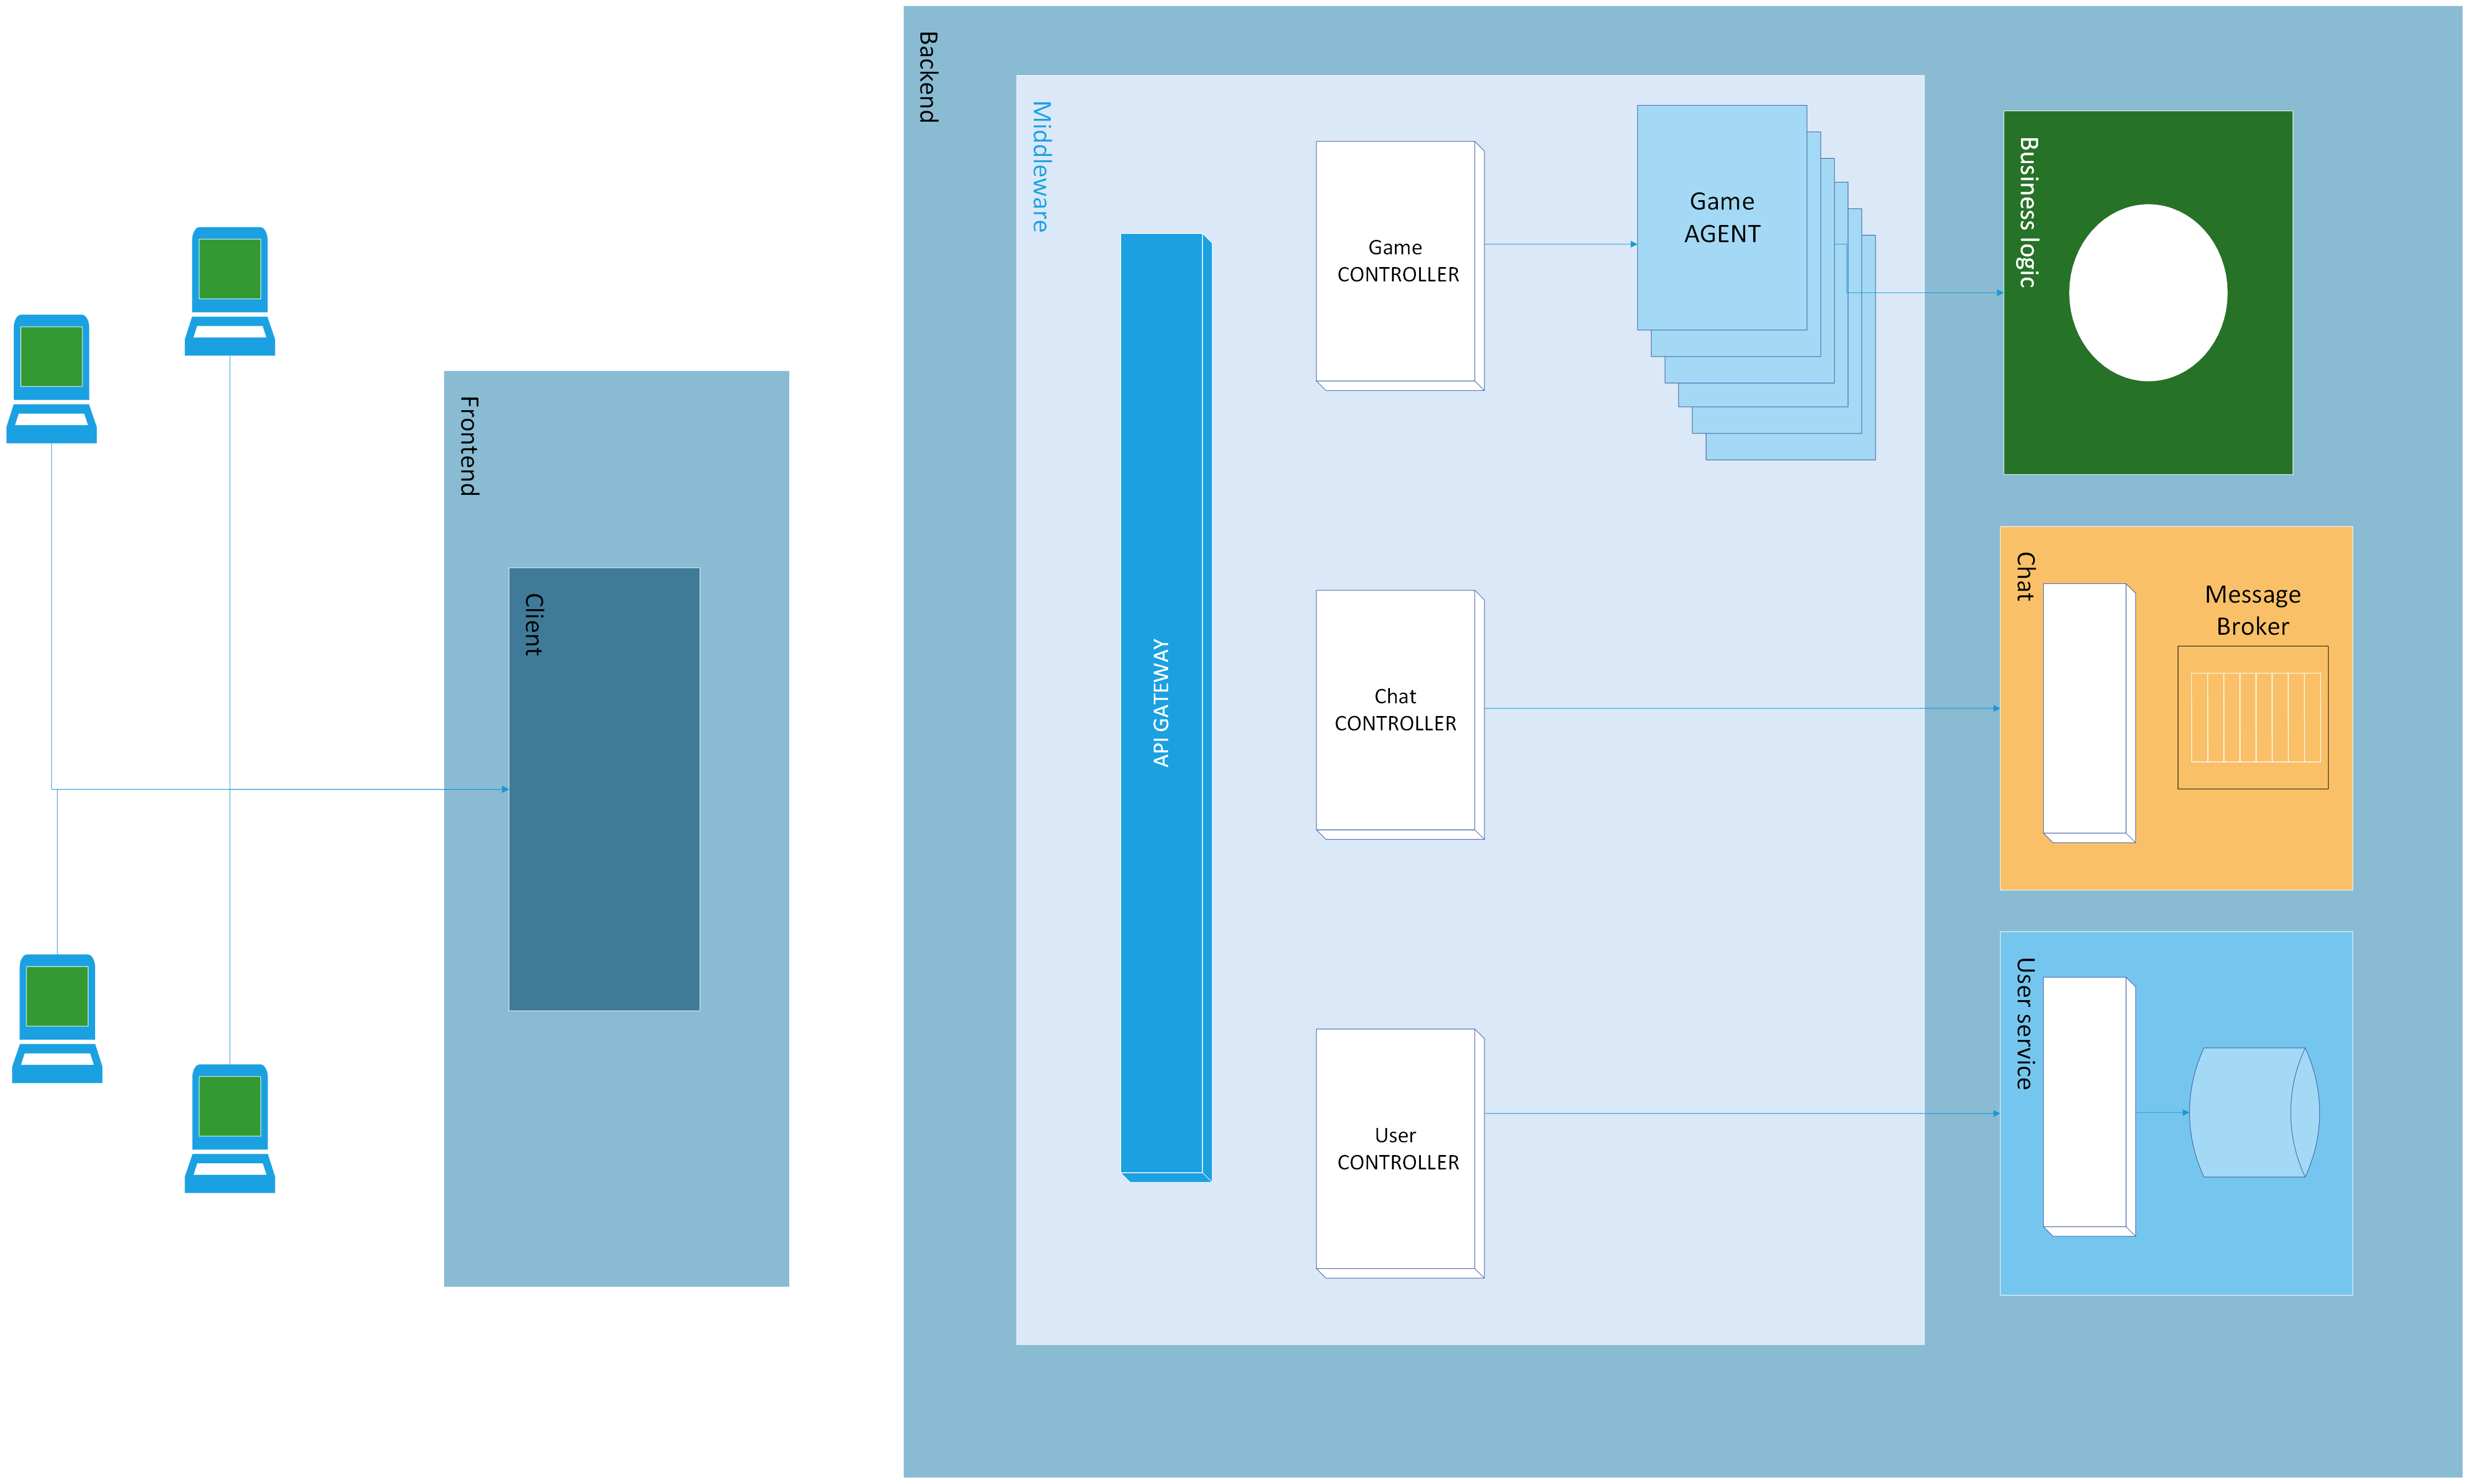
\includegraphics[width=12cm]{report/img/Architecture.png}\\[10.5cm]

\section{Micro-servizi e la loro architettura}

% \subsection{Servizio per la Chat}

% \begin{table}[h!]
%     \centering
%     \caption{Tabella descrittiva Chat Service}
%     \label{tab:chat_serv_table}
%     \begin{tabular}{ll}     
%         \toprule                   
%         Linguaggio & Java \\        
%         Server & Vertx, Swagger \\
%         Librerie & RabbitMQ(vertx) \\
%         Architettura & Agenti vertx \\
%         \bottomrule
%     \end{tabular}
% \end{table}

% 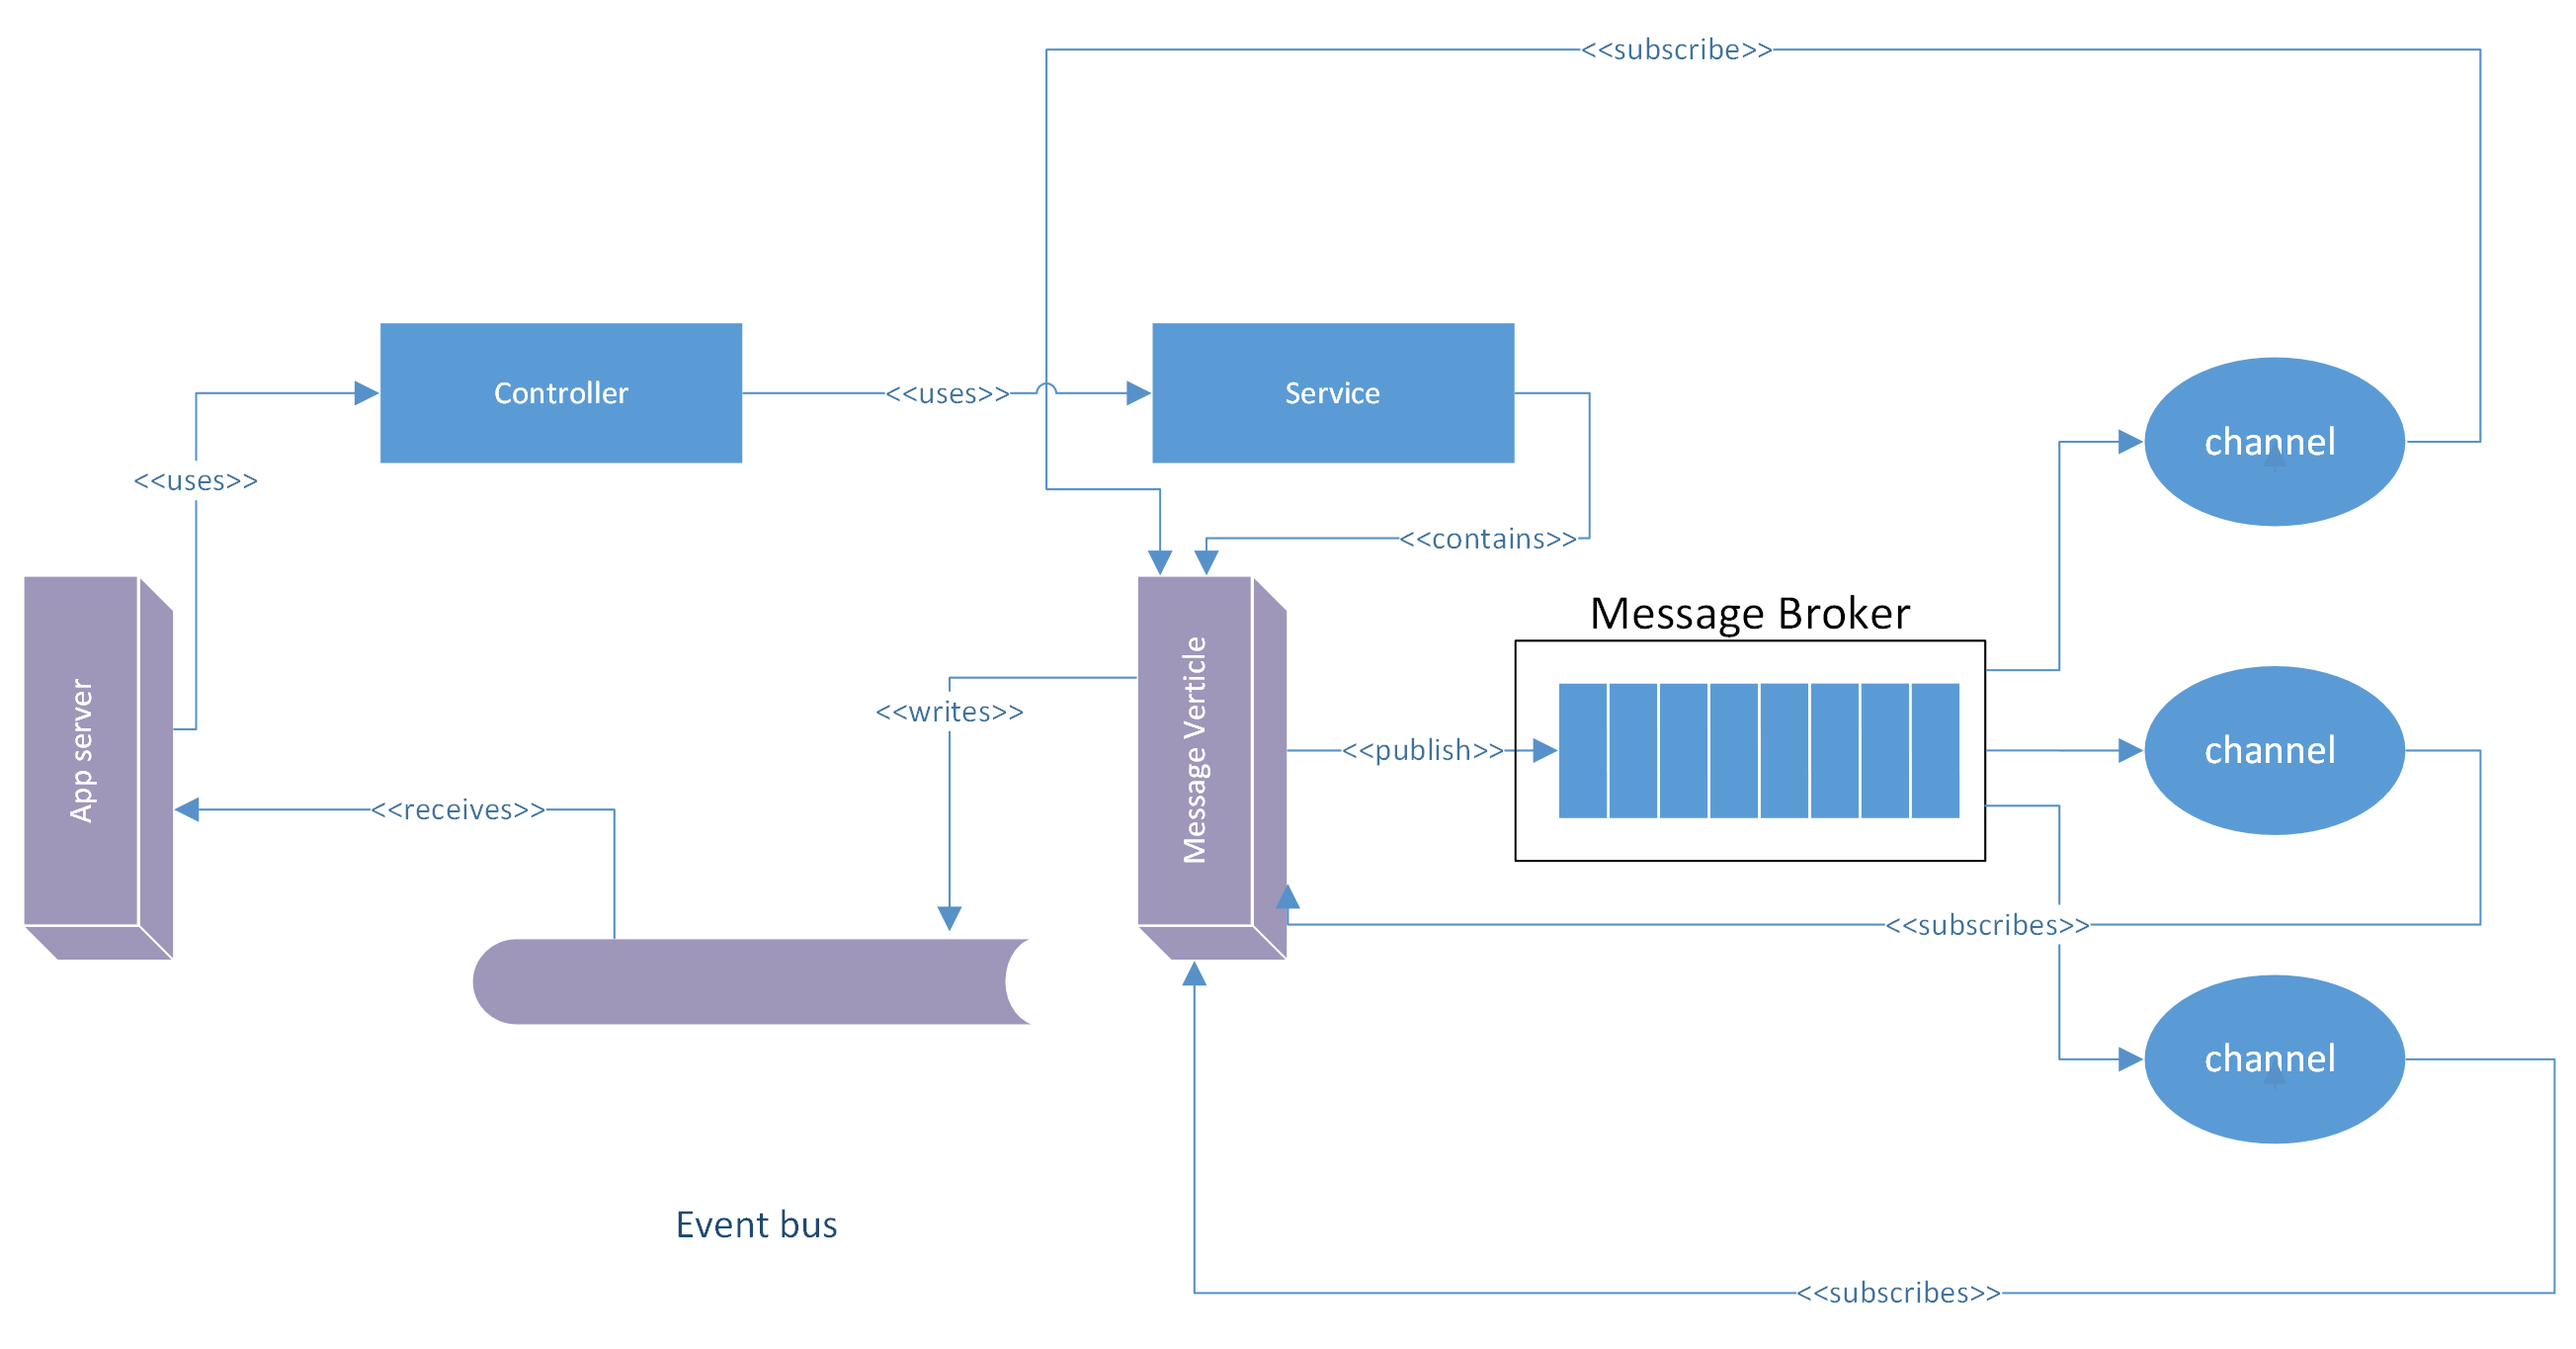
\includegraphics[width=15cm]{report/img/Architettura ChatService.png}\\[10.5cm]

\subsection{Servizio per Gestione Utenti}

\begin{table}[h!]
    \centering
    \caption{Tabella descrittiva User Service}
    \label{tab:user_serv_table}
    \begin{tabular}{ll}     
        \toprule                   
        Linguaggio & Node.JS/TypeScript \\        
        Framework & NestJS   \\                   
        Persistence & Mysql  \\
        Librerie & TypeORM   \\
        Architettura & Model-Controller-service  \\
        \bottomrule
    \end{tabular}
\end{table}


\subsection{Servizio Business Logic}

\begin{table}[h!]
    \centering
    \caption{Tabella descrittiva Business Logic}
    \label{tab:bl_serv_table}
    \begin{tabular}{ll}     
        \toprule                   
        Linguaggio & Node.JS/TypeScript \\        
        Framework & NestJS   \\                   
        Architettura & Model-Controller-service  \\
        \bottomrule
    \end{tabular}
\end{table}

\subsection{Servizio ponte tra i microservizi}


\begin{table}[h!]
    \centering
    \caption{Tabella descrittiva Middleware}
    \label{tab:middleware_serv_table}
    \begin{tabular}{ll}     
        \toprule                   
        Linguaggio & Java \\        
        Server & Vertx \\
        Librerie & RabbitMQ(vertx) \\
        Architettura & Multi-agent, motore di gioco \\
        \bottomrule
    \end{tabular}
\end{table}

\section{[DS/SPE] Perche' i microservizi?}

Ogni microservizio si occupa di gestire un singolo ambito di progetto, il che fa sì che si ottengano ottimi risultati riguardo la qualità e l'affidabilità, la riutilizzabilità, la flessibilità e la scalabilità.
Tutti i componenti sono "loosely coupled", distribuiti in modo indipendente, altamente collaudabili e gestibili e in ambiti reali gestiti da un piccolo team.
Tuttavia, non si tratta di una soluzione definitiva, ha anche degli svantaggi come ad esempio:
\begin{itemize}
    \item la complessità di gestione e la necessità di un'infrastruttura di rete molto complessa.
    \item un'ottima comunicazione di team.
    \item una discreta capacità di astrazione e progettazione di interfaccie di comunicazione che devono essere rispettate da tutti i microservizi.
    \item Non si ha la certezza che l'infrastruttura funzioni correttamente fino a quando tutti i servizi non cooperano tra loro.
\end{itemize}

% \subsection{[SPE] Vantaggi}
% - devops
% - ci 

\subsection{Vantaggi dell'architettura a microservizi}

\subsubsection{Fault Tolerance}

Progettare un sistema completamente privo di errori è un obiettivo decisamente ambizioso e molto difficile da raggiungere. 
Molto più realistico, e inerente al nostro percorso, è progettare un sistema che sia in grado di tollerare, nella giusta misura, gli errori che inevitabilmente si verificheranno. 
La scelta di questa architettura tra i vari vantaggi offre la possibilità di \textbf{isolare parti del sistema}, evitando che gli errori si propaghino in modo incontrollato e che il sistema nel suo complesso vada in crash. 
Ogni sistema opera in modo indipendente e autonomo, con le proprie risorse e la propria logica.
\vspace{1cm}

Lo snodo centrale di comunicazione dei servizi, il middleware, è in grado di gestire le comunicazioni tra i vari microservizi e di garantire che il sistema sia in grado di funzionare anche in caso di guasti.
Purtroppo non esiste alcun progetto senza alcun tipo di \textbf{single point of failure}, o almeno non con le risorse a disposizione di noi studenti, quindi all'interno di questo servizio la 
gestione degli errori dei servizi con cui comunica è gestita, ma di fatto, nel caso in cui il middleware smetta di funzionare, non avendo nessun altro servizio che possa fare da garante 
per il suo corretto funzionamento, tutto il sistema non permetterà, ad esempio, di giocare a nessun gioco.
Questo perché il middleware è il cuore pulsante del sistema; avendo disponibilità di risorse e abbastanza conoscenze in un ambito reale, questo problema ha soluzioni: 
\begin{itemize}
    \item \textbf{Backup del middleware}: avere dei backup dei processi che si occupano di gestire le partite, ma questo significherebbe andare a modificare inevitabilmente 
    la struttura già esistente del servizio.
    \item \textbf{Ridondanza del middleware}: avere molteplici istanze del middleware, preferibilmente 3, di cui una principale e le altre 2 in copia, facendo in modo che
    ogni azione sul middleware principale venga replicata sulle altre due istanze e che quindi, in caso di guasto hardware, le altre copie possano rispondere alle richieste.
\end{itemize}

\subsubsection{Scalabilità}

Nel caso del middleware, la scalabilità è un altro modo per chiamare la duplicazione, ma questo si applica soltanto al middleware, in quanto gli altri microservizi sono realmente scalabili.
Ogni microservizio è in grado di scalare in modo indipendente, in base alle proprie esigenze, e questo permette di avere un sistema che si adatta in modo dinamico alle richieste degli utenti. 
Nella prossima sezione verrà approfondito come il deployment con Docker permetta di scalare i microservizi. L'implementazione di un sistema di load balancing viene fornita
"gratuitamente" da Kubernetes, che permette di bilanciare il carico tra i vari nodi del cluster. 
Qualora il progetto maraffa-online dovesse avere un numero di utenti molto elevato, si potrebbe pensare di scalare il sistema in modo orizzontale, aggiungendo nuovi nodi al cluster, 
e tramite la dovuta configurazione, Kubernetes si occuperebbe di bilanciare il carico tra i vari nodi dei servizi scalabili. 


\subsubsection{Docker}

Suddividere un progetto monolitico in servizi a sé stanti permette di dockerizzare comodamente ogni servizio, e questo consente di avere un sistema facilmente deployabile, versionabile e portabile.
Uno dei requisiti fondamentali del progetto era riuscire a dockerizzare interamente il sistema. Nel caso in cui si volesse fare un deploy su un server remoto, sarebbe sufficiente avere Docker installato, accedere al docker-compose del progetto, settare le corrette variabili d'ambiente e poi il progetto opererebbe in totale autonomia.
Inoltre, utilizzare uno stack permette anche di gestire eventuali failure dei servizi in modo più semplice, poiché Docker consente di avere un sistema fault-tolerant. Se un servizio dovesse andare in crash per qualche motivo inspiegabile, Docker si occuperebbe di riavviarlo in modo autonomo.
L'utilizzo di uno stack permette anche di scalare i servizi in modo più semplice, poiché basta settare il numero di repliche desiderate per un servizio e Docker si occuperà di creare le repliche e di bilanciare il carico tra di esse. Questo è un vantaggio nel caso in cui si voglia scalare il sistema in modo verticale, ovvero aumentando le risorse di un singolo servizio.


\section{Servizi di Business Logic e User Service}

Entrambi questi servizi sono stati realizzati con lo stack NestJS, un framework per Node.js che semplifica la realizzazione di web server e API REST.
Si occupano rispettivamente di gestire la logica di gioco e la gestione degli utenti che vogliono utilizzare il sistema, due core business del progetto.

\subsection{Business Logic}

Questo servizio mantiene al proprio interno tutte le regole del gioco e il calcolo dei punteggi. 
Ha svariati endpoint che permettono al middleware di avere il minor numero possibile di responsabilità, delegando al servizio di business logic le operazioni riguardanti il gioco.

Questa scelta è stata fatta per mantenere il middleware il più leggero possibile e per evitare che si occupi di operazioni non di sua competenza. Inoltre, in futuro sarà possibile aggiungere nuovi giochi modificando il meno possibile il middleware, che dovrà semplicemente occuparsi della gestione delle partite e comunicare tempestivamente con i servizi di business logic in base al gioco scelto.

\subsection{User Service}

Questo servizio gestisce gli utenti, quindi la loro registrazione, autenticazione e gestione dei dati personali.
Anche in questo caso, il middleware delega al servizio di gestione degli utenti le operazioni riguardanti gli utenti, per mantenere il middleware il più leggero possibile e per evitare che si occupi di operazioni non di sua competenza.
Il core di questo servizio è dato dalla combinazione di NestJS e TypeORM, che permettono di gestire in modo semplice e veloce la persistenza dei dati e le operazioni CRUD su un database MySQL.
Oltre alle informazioni degli utenti, il database contiene anche le informazioni riguardanti le partite giocate e le statistiche personali di ogni utente del sistema.

\section{Front-End}

Il front-end è stato realizzato con Angular e si occupa di gestire l'interfaccia grafica e la comunicazione con il middleware.
Sono state realizzate diverse pagine, tra cui la home page, la pagina di registrazione, la pagina di login, la pagina di gioco e la pagina di profilo utente.
Utilizza API REST per comunicare con il middleware e ottenere i dati necessari per il funzionamento del gioco, mentre utilizza WebSockets per la comunicazione in tempo reale con il middleware. 

%TODO altro da dire sui servizi ?

\section{Middleware}

Come già citato, il middleware è il cuore del sistema. L'architettura utilizzata per la gestione delle partite è quella di un multi-agente, in cui ogni agente si occupa di gestire una partita 
e di orchestrare la comunicazione con gli altri servizi, come ad esempio il front-end. Questo core è stato realizzato con Vertx, che è stato utilizzato anche per creare un web-server in Java.

Inoltre, al middleware è collegato un database NoSQL su MongoDB, che viene aggiornato a ogni trick completato dai giocatori per creare uno storico delle partite e salvare le loro decisioni in gioco. 
Questa raccolta di dati sarà parte di uno sviluppo futuro, in cui, dopo aver raccolto una grande quantità di dati di partite, si potrà tentare di creare un modello di machine learning per sviluppare un'intelligenza artificiale che possa giocare al posto di un giocatore umano.

\subsection{Struttura API Gateway}

Il pattern di progettazione utilizzato per la realizzazione del middleware è quello dell'API Gateway, che permette di creare un'interfaccia unica per l'accesso ai vari servizi del sistema.

Nel nostro progetto, il client effettua semplici chiamate verso il middleware, che nei casi necessari effettua chiamate verso altri servizi per svolgere una determinata operazione.
Queste chiamate non sono obbligatoriamente dirette verso il servizio interessato, ma possono anche essere routine che effettuano molteplici chiamate per ottenere il risultato desiderato. 
Ad esempio, nel caso di una partita, considerando l'azione di giocare sul tavolo una carta da parte di un utente, il middleware si occuperà di effettuare alcune chiamate verso il servizio di business
logic per assicurarsi che la carta giocata in quel momento sia valida rispetto alle altre presenti sul tavolo virtuale e di conteggiare effettivamente i punti della mano nel caso in cui tutti i giocatori abbiano giocato una carta. Implementare queste chiamate direttamente nel front-end avrebbe reso il codice molto più complesso e difficile da mantenere, e la gestione di partite multiple sarebbe stata molto più difficile.

Non è stato implementato nessun meccanismo di discovery per la gestione di chiamate verso gli altri servizi, in quanto tutti presenti sullo stesso server e nello stesso stack di Docker, quindi facilmente individuabili sulla rete virtuale creata da Docker.

% \section{Punti comuni tra i servizi}

% \subsection{Swagger}
    \chapter{Interazioni}
\label{ch:interazioni} % This how you label a chapter and the key (e.g., ch:into) will be used to refer this chapter ``Introduction'' later in the report. 
% the key ``ch:into'' can be used with command \ref{ch:intor} to refere this Chapter.
% interazioni tra i componenti, come comunicano, diagrammi d'attività.
% (parlare di api gateway (permette comunicazione tra client esterni con i microservizi, redireziona le richieste ai servizi))

\section{Frontend $ \leftrightarrow $ WebSocket} 

Come precedentemente citato, il middleware è stato implementato con WebSocket per poter comunicare in modo reattivo con il frontend. Queste comunicazioni frontend <-> middleware sono in buona parte scambi di messaggi tramite HTTP, ma in alcuni casi è necessario un canale di comunicazione bidirezionale. Uno degli esempi più "eclatanti" è la dashboard, in cui, in una prima implementazione, era stato utilizzato un polling per aggiornare i dati riguardanti le partite in corso per permettere agli utenti di partecipare. Immaginando uno scenario distribuito in cui ci sono N utenti contemporaneamente connessi al sistema, quella soluzione avrebbe sovraccaricato il sistema. Invece, tramite il canale bidirezionale delle WebSocket, è direttamente il middleware, che al proprio interno ha un servizio che mantiene una mappa dei client connessi, a notificare tramite un'operazione di broadcast tutti i client della creazione di una nuova partita.

\subsection{Chat globale e privata}

Un grande vantaggio dell'uso delle WebSocket sta nella facile implementazione delle chat. Questo sistema richiedeva l'impiego di due diverse chat per permettere la comunicazione tra utenti sia globalmente che all'interno di una singola partita. 
Anche in questo caso, il middleware si occupa di instradare i messaggi alle giuste chat, garantendo la privacy delle conversazioni. Il frontend, invece, si occupa di visualizzare i messaggi e di inviarli al middleware. La gestione della persistenza delle chat è stata implementata tramite l'uso del session storage del browser all'interno del middleware, permettendo di mantenere la chat anche in caso di refresh della pagina.

\subsection{Reattività e aggiornamento in tempo reale}
Tramite l'utilizzo delle WebSocket, è possibile ottenere un aggiornamento in tempo reale delle informazioni, senza dover fare polling continuo al server. Questa tecnologia è stata ampiamente utilizzata nella pagina della partita, permettendo ai client di ricevere aggiornamenti immediati, ad esempio sulle carte giocate da altri giocatori o su eventi scatenati da azioni specifiche, come l'abbandono di un giocatore, la gestione dei punteggi o la conclusione della partita stessa.

\section{Stack Docker $ \rightarrow $ reti interne e IP privati}

Il sistema è stato progettato per essere eseguito su qualsiasi piattaforma e si è arrivati a creare uno stack completo di Docker Compose. Questo ha permesso anche la creazione di reti interne tra i container che vengono utilizzate per la comunicazione tra i servizi. È stato possibile assegnare IP privati ai container, permettendo di non esporre i servizi all'esterno e di mantenere un'architettura più sicura. Tra le variabili d'ambiente che vengono passate ai container c'è anche l'indirizzo del servizio a cui connettersi, e questo indirizzo è il nome del servizio all'interno della rete. Questo permette di non dover modificare il codice ogni volta che si cambia l'indirizzo del servizio a cui connettersi, ma basta modificare il file di configurazione del Docker Compose.
\subsection{Nginx} \label{Nginx}
Per quanto riguarda il frontend, è stato utilizzato Nginx per eseguire l'applicazione all'interno del container e per poterla raggiungere dall'esterno. Per fare ciò è stato necessario configurare Nginx tramite un file di configurazione che ha permesso anche di gestire un'operazione di reverse proxy per indirizzare le chiamate al backend.

\begin{lstlisting}[language=Python, caption={Configurazione Nginx del front-end}, label=list:nginx_frontend]
server {
    listen 80;
    
    location / {
        root /usr/share/nginx/html;
        index index.html index.htm;
        try_files $uri $uri/ /index.html;
    }

    location /api/ {
        proxy_pass "http://${API_HOST}:${API_PORT}/";
        proxy_http_version 1.1;
        proxy_set_header Upgrade $http_upgrade;
        proxy_set_header Connection 'upgrade';
        proxy_set_header Host $host;
        proxy_cache_bypass $http_upgrade;
    }
}
\end{lstlisting}
La scelta di Nginx è stata fatta soprattutto per la sicurezza nel "mascherare" le chiamate fatte al backend, in modo da non esporre l'indirizzo del servizio all'esterno e poter superare eventuali problemi di CORS. L'indirizzo del backend è stato configurato anch'esso tramite variabili d'ambiente, in modo da poterlo cambiare facilmente in base all'ambiente in cui si trova il container, e queste variabili vengono sostituite a seconda dell'ambiente di deploy in cui l'applicativo Angular viene eseguito.

% %%%%%%%%%%%%%%%%%%%%%%%%%%%%%%%%%%%%%%%%%%%%%%%%%%%%%%%%%%%%%%%%%%%%%%%%%%%%%%%%%%%
% \section{Problem statement}
% \label{sec:intro_prob_art}
% This section describes the investigated problem in detail. You can also have a separate chapter on ``Problem articulation.''  For some projects, you may have a section like ``Research question(s)'' or ``Research Hypothesis'' instead of a section on ``Problem statement.'

% %%%%%%%%%%%%%%%%%%%%%%%%%%%%%%%%%%%%%%%%%%%%%%%%%%%%%%%%%%%%%%%%%%%%%%%%%%%%%%%%%%%
% \section{Aims and objectives}
% \label{sec:intro_aims_obj}
% Describe the ``aims and objectives'' of your project. 

% \textbf{Aims:} The aims tell a read what you want/hope to achieve at the end of the project. The  aims define your intent/purpose in general terms.  

% \textbf{Objectives:} The objectives are a set of tasks you would perform in order to achieve the defined aims. The objective statements have to be specific and measurable through the results and outcome of the project.


% %%%%%%%%%%%%%%%%%%%%%%%%%%%%%%%%%%%%%%%%%%%%%%%%%%%%%%%%%%%%%%%%%%%%%%%%%%%%%%%%%%%
% \section{Solution approach}
% \label{sec:intro_sol} % label of Org section
% Briefly describe the solution approach and the methodology applied in solving the set aims and objectives.

% Depending on the project, you may like to alter the ``heading'' of this section. Check with you supervisor. Also, check what subsection or any other section that can be added in or removed from this template.

% \subsection{A subsection 1}
% \label{sec:intro_some_sub1}
% You may or may not need subsections here. Depending on your project's needs, add two or more subsection(s). A section takes at least two subsections. 

% \subsection{A subsection 2}
% \label{sec:intro_some_sub2}
% Depending on your project's needs, add more section(s) and subsection(s).

% \subsubsection{A subsection 1 of a subsection}
% \label{sec:intro_some_subsub1}
% The command \textbackslash subsubsection\{\} creates a paragraph heading in \LaTeX.

% \subsubsection{A subsection 2 of a subsection}
% \label{sec:intro_some_subsub2}
% Write your text here...

% %%%%%%%%%%%%%%%%%%%%%%%%%%%%%%%%%%%%%%%%%%%%%%%%%%%%%%%%%%%%%%%%%%%%%%%%%%%%%%%%%%%
% \section{Summary of contributions and achievements} %  use this section 
% \label{sec:intro_sum_results} % label of summary of results
% Describe clearly what you have done/created/achieved and what the major results and their implications are. 


% %%%%%%%%%%%%%%%%%%%%%%%%%%%%%%%%%%%%%%%%%%%%%%%%%%%%%%%%%%%%%%%%%%%%%%%%%%%%%%%%%%%
% \section{Organization of the report} %  use this section
% \label{sec:intro_org} % label of Org section
% Describe the outline of the rest of the report here. Let the reader know what to expect ahead in the report. Describe how you have organized your report. 

% \textbf{Example: how to refer a chapter, section, subsection}. This report is organised into seven chapters. Chapter~\ref{ch:lit_rev} details the literature review of this project. In Section~\ref{ch:method}...  % and so on.

% \textbf{Note:}  Take care of the word like ``Chapter,'' ``Section,'' ``Figure'' etc. before the \LaTeX command \textbackslash ref\{\}. Otherwise, a  sentence will be confusing. For example, In \ref{ch:lit_rev} literature review is described. In this sentence, the word ``Chapter'' is missing. Therefore, a reader would not know whether 2 is for a Chapter or a Section or a Figure.

    \chapter{Implementazione}
\label{ch:implementazione} % This how you label a chapter and the key (e.g., ch:into) will be used to refer this chapter ``Introduction'' later in the report. 
% the key ``ch:into'' can be used with command \ref{ch:intor} to refere this Chapter.
parla di decomposizione delle funzionalità in microservizi
dipendenze minime tra i servizi
reattività agli eventi
\section{Tecnologie}
(swagger, postman, autogenerazione javadoc?, rabbitMQ, JWT per autenticazione utenti,
 docker, nodejs, typescript, mongodb, jest, angular, figma, ...)
\subsection{Swagger - OpenAPI}

Uno dei requisiti fondamentali di questo progetto è stata la documentazione delle API.
Per fare ciò è stato utilizzato Swagger, un framework open-source che permette di descrivere, produrre e consumare servizi web RESTful. 
Swagger permette di testare le API direttamente dalla documentazione, grazie a un'interfaccia grafica che consente di inviare richieste e visualizzare le risposte.

\vspace{1cm}

Per i servizi creati in Node.js è stata utilizzata una libreria ad hoc, in grado di generare la documentazione automaticamente tramite i corretti decoratori.
Al contrario, per i servizi in Java non esiste alcuna libreria in grado di generare automaticamente la documentazione API a partire dai metodi esposti, quindi è stata creata manualmente.
Grazie a un lavoro preliminare open-source svolto da \href{https://github.com/anupsaund}{\underline{Anup Saund}} sulla sua repository \href{https://github.com/anupsaund/vertx-auto-swagger}{\underline{Vertx auto swagger}}, è stato possibile creare automaticamente un file HTML contenente la documentazione delle API esposte dai servizi in Java. 
Purtroppo, questo file non era in grado di aggiornarsi automaticamente in caso di modifiche alle rotte, quindi è stato necessario adattarlo per renderlo più flessibile e adatto al nostro progetto.

\vspace{1cm}

Vertx è una libreria davvero completa e ben strutturata. È stato possibile creare un Router in grado di gestire tutte le rotte del progetto in Java utilizzando una semplice classe astratta che ha definito tutti i metodi utilizzati nel progetto, tramite la quale si è potuto razionalizzare il codice e creare dinamicamente la funzionalità richiesta.

\begin{lstlisting}[language=Java, caption={Semplice interfaccia per le rotte HTTP}, label=list:java_swagger_interface]
package httpRest;

import io.vertx.core.Handler;
import io.vertx.core.http.HttpMethod;
import io.vertx.ext.web.RoutingContext;

public interface IRouteResponse {
    HttpMethod getMethod();
    String getRoute();
    Handler<RoutingContext> getHandler();
}
\end{lstlisting}

La parte realmente complicata è stata fare in modo che le annotazioni presenti nel codice sorgente venissero lette e trasformate in un file JSON che rappresentasse correttamente la documentazione delle API. 
Dopo alcuni tentativi, è stato possibile automatizzare anche questa operazione.

\begin{lstlisting}[language=Java, caption={Aggiunta dei moduli delle classi contenenti rotte HTTP}, label=list:java_swagger_modules]
final ImmutableSet<ClassPath.ClassInfo> modelClasses = ImmutableSet.<ClassPath.ClassInfo>builder()
        .addAll(this.getClassesInPackage("game"))
        .addAll(this.getClassesInPackage("userModule"))
        .addAll(this.getClassesInPackage("BLManagement"))
        .addAll(this.getClassesInPackage("chatModule"))
        .build();
\end{lstlisting}

\vspace{1cm}

Java permette di creare oggetti molto complessi, diversi dai JSON / object solitamente utilizzati in JavaScript. Era fondamentale poter adoperare questi schemi per avere una documentazione ricca e per poter testare velocemente le API senza utilizzare necessariamente un client come Postman. 

Infine, per poter mostrare correttamente la documentazione, è stato necessario creare un file HTML che permettesse di visualizzare la documentazione in modo chiaro e ordinato. Questo file statico, presente nella repository del progetto, utilizza come fonte il file JSON di OpenAPI che viene rigenerato a ogni build del progetto, in modo da avere sempre la documentazione aggiornata.

\subsection{Postman}


\subsection{Log automatici}

Il servizio core del sistema è il middleware e per poterlo monitorare è stato necessario implementare un sistema di log automatici. Tenere traccia di tutte le operazioni è un compito molto complesso e avrebbe reso difficile un eventuale debug su un software in produzione quindi 
grazie a Vertx, che offre gratuitamente un logger e alla libreria \href{https://mvnrepository.com/artifact/ch.qos.logback/logback-classic}{\underline{LogBack}} i dei servizi più importanti sono trascritti su file .log in modo da poterli analizzare in caso di problemi.

Questo sistema poi si è evoluto grazie ad una configurazione di logback in un file xml tramite il quale è possibile personalizzare completamente il sistema di log, decidendo quali package loggare, in quali file trascriverli, scegliere addirittura il livello di log (info, debug, error, ecc...)
ed infine attuare un sistema di log rotate secondo il quale i log oltre una certa dimensione impostata da questa configurazione vengono compressi e rinominati in modo da non occupare troppo spazio ed è possible anche settare il numero di questi file compressi da mantenere.

\vspace{1cm}

Questo sistema si adatta perfettamente ad un software dockerizzabile che ha montato un volume relativo alla cartella /log, che può anche essere un volume remoto, da cui poter consultare velocemente i log in caso di problemi.


\section{Parte di distribuiti che non so dove mettere, sta nell'impl? p.s. dargli un nome decente}
FAULT DETECTION (con node nel cluster, nel nostro caso?)/TOLLERANCE
SCALABILITà?
verificare la scalabilità orizzontale (aumento richieste in un periodo)?
PERSISTENZA
CONSISTENZA
AFFIDABILITà
FAULTS (GIOCATORE SI DISCONNETTE NEL MEZZO DELLA PARTITA)
IL SISTEMA SI BLOCCA IN CASO DI ERRORI?
**GUARDA L'ESEMPIO DI POLITICHE AUTOVALUTAZIONE NELL'ANALISI**

monitoraggio per osservare stato attuale sistema (mi sa che noi non l'abbiamo)
\section{Screen}
\section{Optional(Mockup)}
% %%%%%%%%%%%%%%%%%%%%%%%%%%%%%%%%%%%%%%%%%%%%%%%%%%%%%%%%%%%%%%%%%%%%%%%%%%%%%%%%%%%
% \section{Problem statement}
% \label{sec:intro_prob_art}
% This section describes the investigated problem in detail. You can also have a separate chapter on ``Problem articulation.''  For some projects, you may have a section like ``Research question(s)'' or ``Research Hypothesis'' instead of a section on ``Problem statement.'

% %%%%%%%%%%%%%%%%%%%%%%%%%%%%%%%%%%%%%%%%%%%%%%%%%%%%%%%%%%%%%%%%%%%%%%%%%%%%%%%%%%%
% \section{Aims and objectives}
% \label{sec:intro_aims_obj}
% Describe the ``aims and objectives'' of your project. 

% \textbf{Aims:} The aims tell a read what you want/hope to achieve at the end of the project. The  aims define your intent/purpose in general terms.  

% \textbf{Objectives:} The objectives are a set of tasks you would perform in order to achieve the defined aims. The objective statements have to be specific and measurable through the results and outcome of the project.


% %%%%%%%%%%%%%%%%%%%%%%%%%%%%%%%%%%%%%%%%%%%%%%%%%%%%%%%%%%%%%%%%%%%%%%%%%%%%%%%%%%%
% \section{Solution approach}
% \label{sec:intro_sol} % label of Org section
% Briefly describe the solution approach and the methodology applied in solving the set aims and objectives.

% Depending on the project, you may like to alter the ``heading'' of this section. Check with you supervisor. Also, check what subsection or any other section that can be added in or removed from this template.

% \subsection{A subsection 1}
% \label{sec:intro_some_sub1}
% You may or may not need subsections here. Depending on your project's needs, add two or more subsection(s). A section takes at least two subsections. 

% \subsection{A subsection 2}
% \label{sec:intro_some_sub2}
% Depending on your project's needs, add more section(s) and subsection(s).

% \subsubsection{A subsection 1 of a subsection}
% \label{sec:intro_some_subsub1}
% The command \textbackslash subsubsection\{\} creates a paragraph heading in \LaTeX.

% \subsubsection{A subsection 2 of a subsection}
% \label{sec:intro_some_subsub2}
% Write your text here...

% %%%%%%%%%%%%%%%%%%%%%%%%%%%%%%%%%%%%%%%%%%%%%%%%%%%%%%%%%%%%%%%%%%%%%%%%%%%%%%%%%%%
% \section{Summary of contributions and achievements} %  use this section 
% \label{sec:intro_sum_results} % label of summary of results
% Describe clearly what you have done/created/achieved and what the major results and their implications are. 


% %%%%%%%%%%%%%%%%%%%%%%%%%%%%%%%%%%%%%%%%%%%%%%%%%%%%%%%%%%%%%%%%%%%%%%%%%%%%%%%%%%%
% \section{Organization of the report} %  use this section
% \label{sec:intro_org} % label of Org section
% Describe the outline of the rest of the report here. Let the reader know what to expect ahead in the report. Describe how you have organized your report. 

% \textbf{Example: how to refer a chapter, section, subsection}. This report is organised into seven chapters. Chapter~\ref{ch:lit_rev} details the literature review of this project. In Section~\ref{ch:method}...  % and so on.

% \textbf{Note:}  Take care of the word like ``Chapter,'' ``Section,'' ``Figure'' etc. before the \LaTeX command \textbackslash ref\{\}. Otherwise, a  sentence will be confusing. For example, In \ref{ch:lit_rev} literature review is described. In this sentence, the word ``Chapter'' is missing. Therefore, a reader would not know whether 2 is for a Chapter or a Section or a Figure.

    \chapter{DevOps}
\label{ch:DevOps} % This how you label a chapter and the key (e.g., ch:into) will be used to refer this chapter ``Introduction'' later in the report. 
% the key ``ch:into'' can be used with command \ref{ch:intor} to refere this Chapter.
% \section{Git wordkflow}
\section{DVCS}

Come strumento di controllo di versione è stato scelto git, sono state adottate le seguenti best practices o git policy per garantire un flusso di lavoro coerente e prevenire conflitti di merge.
% La Git Policy rappresenta un insieme di linee guida e regole che governano l'uso di Git all'interno di un team di sviluppo. 
% Queste politiche sono fondamentali per garantire un flusso di lavoro coerente, prevenire conflitti di merge e mantenere una storia del codice chiara e facilmente navigabile. 

\subsection{Struttura dei Branch}

Una delle componenti principali della Git Policy è la gestione dei branch. La struttura tipica prevede almeno tre tipi di branch:
- \textbf{Master/Main:} Questo è il branch principale che contiene il codice di produzione. Ogni commit su questo branch dovrebbe essere stabile e pronto per il rilascio. Questo branch e stato protetto per evitare commit diretti, richiedendo quindi una revisione per ogni operazione di merge.
- \textbf{Develop:} Qui viene integrato il lavoro di sviluppo corrente. È il branch dove confluiscono le feature prima di essere preparate per il rilascio. Questo branch dovrebbe essere costantemente aggiornato e testato per assicurare che sia in uno stato pronto per la produzione.
- \textbf{Feature Branches:} Utilizzati per lo sviluppo di nuove funzionalità. Ogni feature branch deve derivare da `develop` e, una volta completata la feature, viene reintegrato in `develop` tramite una pull request.


% \subsection{Commit e Messaggi di Commit}

% La pratica adottata per i commit è stata quella di effettuare commit frequenti e significativi.
% Per facilitare la comprensione di ogni commit si è adotatto lo standard : \href{https://www.conventionalcommits.org/en/v1.0.0/}{Conventional Commits}, che divide i commit in categorie come `fix`, `feat`, `docs`, `style`, `refactor`, `test`, `chore`, `ci`, `perf`, `build`, `revert`. 

\subsection{Conventional commits}
La pratica adottata per i commit è stata quella di effettuare commit frequenti e significativi.

In ogni repo è stato adottato un sistema standard per scrivere i commit:  i conventional commit. In questo modo i commit risultano più chiari e facilmente leggibili. 
Riportiamo di seguito la nomenclatura usata:
\begin{itemize}
    \item \textbf{fix:} per i commit che risolvono un bug
    \item \textbf{feat:} per i commit che aggiungono una nuova feature
    \item \textbf{refactor:} per i commit che migliorano il codice senza aggiungere nuove funzionalità
    \item \textbf{docs:} per i commit che riguardano la documentazione
    \item \textbf{style:} per i commit che riguardano la formattazione del codice
    \item \textbf{test:} per i commit che riguardano i test
    \item \textbf{ci:} per i commit che riguardano la Continuous Integration
\end{itemize}
Inoltre sono evidenziati i breaking changes per le modifiche non più compatibili con le versioni precedenti.
La stessa nomenclatura viene utilizzata anche nel changelog.


\section{Issue template}
Il codice è open source ed è incoraggiata la collaborazione anche grazie alla presenza, in ogni repository, di template con i quali un utente può consigliare nuove feature,
segnalare un bug o suggerire un'implementazione alternativa. Sono estremamente utili per ricevere feedback dagli utenti e monitorare gli eventuali bug.

\section{Build automation}
Abbiamo deciso di implementare ogni servizio in una repository diversa. La repository fornita è un contenitore di tutte le singole repository dei servizi.
Per ogni repository è stata implementata una build automation specifica. \\
In questo modo si riesce a automatizzare i processi di build, test e deploy, ottenendo diversi vantaggi:
\begin{itemize}
    \item si riduce drasticamente il tempo per la compilazione del codice
    \item ogni volta i passaggi verranno eseguiti allo stesso modo ottenendo, quindi, riproducibilità
    \item si identificano facilmente i problemi grazie al sistema di stampe a video che si ottiene durante l'esecuzione delle GitHub Actions
    \item minimizzazione degli errori umani
    \item garantisce il continuous deployment 
\end{itemize}


\subsection{UserManagementMaraffa e BusinessLogic:} Essendo le due repository estremamente simili e avendo entrambe un ambiente in node.js, è stato implementato un workflow pressochè analogo. Questo workflow reagisce all'evento push sul main branch, e pull request sui branch main e develop 
e sono stati implementati 3 job: build, test e deploy.
Dopo una checkout iniziale (fetch-depth è 0 in quanto il changelog necessita di tutta la history dei commit),
 viene creata una cache per permettere ai job di comunicare tra loro. Successivamente alla build il sistema viene testato
  (in entrambi i casi viene usata l'action di yarn) e infine viene effettuato il deploy del servizio containerizzato
 Nel quale viene effettuato il chekout, si configura il nome del progetto e si configura la versione della build.
 Se il commit viene effettuato sul main si configura il nome del tag e la versione a "LATEST", nel caso non fosse nel main viene configurata la versione a "develop".
  Infine si effettua il login al Github container registry, la build e la push dell'immagine sul registro. L'immagine viene configurata in modo parametrico con delle variabili d'ambiente e il nome viene trasformato in minuscolo. 

\subsection{MiddlewareMaraffa:} 
Quando viene effettuata una pull request sul branch develop ed è di tipo closed
(non sta progredendo e quindi l’esecuzione non è in corso) il workflow del Middleware viene attivato.
Anch'esso è costituito da tre jobs: build, test e deploy.
Come prima cosa nella build, viene eseguito il checkout, effettuato il setup di Java e Gradle. Infine viene effettuata la 
build di Gradle.
Nel job del test si effettua il login al database di MongoDB. Password e username vengono passati tramite i secrets. Successivamente
si prosegue con checkout, setup di Java utilizzando la cache per utilizzare la build di Gradle svolta precedentemente e 
infine si esegue il test con gradlew.
Per quanto riguarda il deploy, si effettua il checkout utilizzando un token salvato all'interno di un secret. La parte
restante coincide con quella delle repository precedenti.
% push su main, pull request su main e develop
% build e test se pullrequest.merge = true 

% Parte finale 


\begin{itemize}
\item \textbf{ChatServer:} Il servizio è sviluppato in un ambiente Java, pertanto dopo aver effettuato il checkout nel job build and test,  si effettua il set-up di Java (distribuzione: temurin, versione 20). Viene svolto il set-up di Gradle, in cui viene usata un'action per la build e creata una cache. Inoltre viene aggiunto un commento con un riassunto dei risultati dei job  alla pull request, il cui valore è impostato a "on-failure". Si noti che il suo valore di default è "never"; se fosse "always", si potrebbero verificare scenari indesiderati. Il riassunto dei risultati dei job risulta particolarmente utile: un utente che vuole esaminare la pull request riesce a comprendere lo stato dei job (se sono stati eseguiti correttamente oppure no) in modo leggibile e intuitivo. Successivamente si effettua il deploy del container di rabbitMQ se l'evento è una pull request oppure se è una push sul master o se la stringa con il riferimento a github contiene "tags/v". Infine se tutti il job da cui dipende (build-and-test) non è fallito e non è stato interrotto. Con l'istruzione run si verifica che non ci siano stati dei fallimenti nel job deploy and test.

\item \textbf{FrontendMaraffa:} //TODO
Sarebbe figo spiegare come i nostri workflow hanno ridotto i conflitti di integrazione, il rilevamento precoce di bug e i problemi di compatibilità.

\end{itemize}
\section{Continuous integration}
Per migliorare la qualità del software e velocizzare il processo di sviluppo, è stata implementata la Continuous Integration.
Questa pratica permette di integrare il codice frequentemente, evitando possibili rischi d'integrazione e consetendo 
l'esecuzione di test automatici. Grazie al sistema di notifiche, inoltre, è possibile ricevere feedback immediato sullo stato delle Github Actions,
per accertarsi che sia sempre tutto funzionante e non siano stati introdotti bug. Mantenendo il sistema continuamente monitorato,
si migliora anche l'effiicienza e la collaborazione tra i membri del team.
% -ci (GHA, deploy pages, usato due servizi di hosting github e gitlab (per copia all'intero di repo di magnani))


% %%%%%%%%%%%%%%%%%%%%%%%%%%%%%%%%%%%%%%%%%%%%%%%%%%%%%%%%%%%%%%%%%%%%%%%%%%%%%%%%%%%
% \section{Problem statement}
% \label{sec:intro_prob_art}
% This section describes the investigated problem in detail. You can also have a separate chapter on ``Problem articulation.''  For some projects, you may have a section like ``Research question(s)'' or ``Research Hypothesis'' instead of a section on ``Problem statement.'

% %%%%%%%%%%%%%%%%%%%%%%%%%%%%%%%%%%%%%%%%%%%%%%%%%%%%%%%%%%%%%%%%%%%%%%%%%%%%%%%%%%%
% \section{Aims and objectives}
% \label{sec:intro_aims_obj}
% Describe the ``aims and objectives'' of your project. 

% \textbf{Aims:} The aims tell a read what you want/hope to achieve at the end of the project. The  aims define your intent/purpose in general terms.  

% \textbf{Objectives:} The objectives are a set of tasks you would perform in order to achieve the defined aims. The objective statements have to be specific and measurable through the results and outcome of the project.


% %%%%%%%%%%%%%%%%%%%%%%%%%%%%%%%%%%%%%%%%%%%%%%%%%%%%%%%%%%%%%%%%%%%%%%%%%%%%%%%%%%%
% \section{Solution approach}
% \label{sec:intro_sol} % label of Org section
% Briefly describe the solution approach and the methodology applied in solving the set aims and objectives.

% Depending on the project, you may like to alter the ``heading'' of this section. Check with you supervisor. Also, check what subsection or any other section that can be added in or removed from this template.

% \subsection{A subsection 1}
% \label{sec:intro_some_sub1}
% You may or may not need subsections here. Depending on your project's needs, add two or more subsection(s). A section takes at least two subsections. 

% \subsection{A subsection 2}
% \label{sec:intro_some_sub2}
% Depending on your project's needs, add more section(s) and subsection(s).

% \subsubsection{A subsection 1 of a subsection}
% \label{sec:intro_some_subsub1}
% The command \textbackslash subsubsection\{\} creates a paragraph heading in \LaTeX.

% \subsubsection{A subsection 2 of a subsection}
% \label{sec:intro_some_subsub2}
% Write your text here...

% %%%%%%%%%%%%%%%%%%%%%%%%%%%%%%%%%%%%%%%%%%%%%%%%%%%%%%%%%%%%%%%%%%%%%%%%%%%%%%%%%%%
% \section{Summary of contributions and achievements} %  use this section 
% \label{sec:intro_sum_results} % label of summary of results
% Describe clearly what you have done/created/achieved and what the major results and their implications are. 


% %%%%%%%%%%%%%%%%%%%%%%%%%%%%%%%%%%%%%%%%%%%%%%%%%%%%%%%%%%%%%%%%%%%%%%%%%%%%%%%%%%%
% \section{Organization of the report} %  use this section
% \label{sec:intro_org} % label of Org section
% Describe the outline of the rest of the report here. Let the reader know what to expect ahead in the report. Describe how you have organized your report. 

% \textbf{Example: how to refer a chapter, section, subsection}. This report is organised into seven chapters. Chapter~\ref{ch:lit_rev} details the literature review of this project. In Section~\ref{ch:method}...  % and so on.

% \textbf{Note:}  Take care of the word like ``Chapter,'' ``Section,'' ``Figure'' etc. before the \LaTeX command \textbackslash ref\{\}. Otherwise, a  sentence will be confusing. For example, In \ref{ch:lit_rev} literature review is described. In this sentence, the word ``Chapter'' is missing. Therefore, a reader would not know whether 2 is for a Chapter or a Section or a Figure.

    % replace all text with your own text.
% in this template few examples are mention
\chapter{Validazione}
\label{ch:validazione} % Label for method chapter

\section{Test} 

Per ogni servizio in questo sistema è stato adottato, ove possibile, il paradigma di programmazione TDD, cioè Test Driven Development. Questo approccio prevede che i test siano scritti prima del codice, in modo da guidare lo sviluppo e garantire che il codice prodotto soddisfi i requisiti specificati.
Le operazioni di testing sono stata implementate con Jest per quanto riguarda i servizi che usano Node.js, generando di fatto un report abbastanza comprensibile. Il componente middleware, scritto in Java, invece, generava risultati di test non così chiari. Per modificare questo comportamento, è stata introdotta una dipendenza nel build Gradle che permette di avere un report più dettagliato e comprensibile. 
La libreria \href{https://plugins.gradle.org/plugin/com.adarshr.test-logger}{\underline{Test Logger}}, tramite una piccola configurazione nel file build.gradle come qui riportata, ha soddisfatto le nostre esigenze.

\begin{lstlisting}[language=Java, caption={Test logger}, label=list:gradle_testlogger]
import com.adarshr.gradle.testlogger.TestLoggerExtension
import com.adarshr.gradle.testlogger.TestLoggerPlugin
import com.adarshr.gradle.testlogger.theme.ThemeType

testlogger {
    theme = ThemeType.MOCHA
    showExceptions = true
    showStackTraces = true
    showFullStackTraces = false
    showCauses = true
    slowThreshold = 2000
    showSummary = true
    showSimpleNames = false
    showPassed = true
    showSkipped = true
    showFailed = true
    showOnlySlow = false
    showStandardStreams = false
    showPassedStandardStreams = true
    showSkippedStandardStreams = true
    showFailedStandardStreams = true
    logLevel = LogLevel.LIFECYCLE
}
\end{lstlisting}
\vspace{1cm}

L'architettura dei componenti si può riassumere in questo modo:
\begin{itemize}
	\item \textbf{Classi controller}: che hanno la funzione di esporre le rotte e di contenere al loro interno classi di servizio.
	\item \textbf{Classi di servizio}: che contengono la logica di business.
\end{itemize}

I test vengono quindi eseguiti sulle classi di servizio, andando a testare la logica di business e non le funzioni. Questo approccio permette di avere una copertura maggiore del codice e di garantire che la logica di business sia corretta.
Un esempio di test su una classe di servizio, prendendo come esempio il componente userManagement, rende chiaro il concetto.

Questo componente di fatto svolge due funzioni ben distinte:
\begin{itemize}
	\item Collegarsi a un database MySQL e fare delle operazioni CRUD su tabelle di utenti e le loro rispettive statistiche. 
	\item Gestire la registrazione e l'autenticazione degli utenti.
\end{itemize}

La parte di testing quindi non va assolutamente a verificare che la connessione al database funzioni, ma che le operazioni CRUD siano corrette e che la registrazione e l'autenticazione degli utenti avvengano correttamente, così come l'aggiornamento delle statistiche.

\vspace{0.5cm}

Avendo scelto un'architettura a microservizi, è stato necessario testare anche il corretto funzionamento delle comunicazioni tra i servizi. Per fare ciò, è stato necessario creare dei test di integrazione che verificassero il corretto funzionamento delle API esposte dai servizi. 
Questi test sono stati implementati nel componente middleware che, come sicuramente si ricorderà, ha il compito di mettere in comunicazione i servizi tra di loro e con il frontend.


\subsection{Testing asincrono}

Durante la scrittura dei test all'interno del servizio in Java, alcune operazioni erano asincrone e quindi è stato necessario attendere che queste operazioni terminassero prima di poter eseguire i test e validarli.
Per fare ciò, la normale struttura di test fornita da Vertx in un primo tentativo non era sufficente, la classica stuttura dei test è la seguente.

\begin{lstlisting}[language=Java, caption={Standard Vertx test}, label=list:test_std_vertx]
	@Test
	public void createGameTest(final VertxTestContext context) {
		final JsonObject gameResponse = this.gameService.createGame(MARAFFA_PLAYERS, TEST_USER, EXPECTED_SCORE, GAME_MODE.toString(), PASSWORD);
		Assertions.assertEquals(UUID_SIZE, gameResponse.getString(Constants.GAME_ID).length()); // Assuming UUID is 36
		context.completeNow();
	}
\end{lstlisting}

Per risolvere questo problema sono stati utilizzati:
\begin{itemize}
\item il decoratore fornito da junit jupiter \textit{@Timeout} che permette di aspettare un tempo definito prima di fallire automaticamente il test, per poter ovviare al problema di asincronicità con servizi esterni al componente stesso che non "rispondono alla chiamata"
\item l'utilizzo asincrono del VertxTestContext, che permette di completare il test solo quando tutte le operazioni asincrone sono state completate.
\item una struttura di risposta, all'interno dei servizi con cui il middleware comunica che permette di inviduare errori tramite la chiave error in caso di fallimento contenuta all'interno del JSON di risposta. Il test non può accedere alla response di una chiamata HTTP che normalmente avrebbe
uno status code 200 in caso di successo e quindi si è ricorsi a questo espendiente per individuare errori nei dati che sarebbero stati inviati al servizio.
\end{itemize}
Come è possibile vedere nell test riportato seguendo questi due accorgimenti, è possibile testare correttamente le operazioni asincrone.

\begin{lstlisting}[language=Java, caption={Vertx test Asincrono}, label=list:test_async_vertx]
	@Timeout(value = 10, unit = TimeUnit.SECONDS)
	@Test
	public void testgetShuffledDeckOK(final VertxTestContext context) {
		final JsonObject gameResponse = this.gameService.createGame(4, TEST_USER, 41,
				GameMode.CLASSIC.toString(), PASSWORD);
		this.businessLogicController
				.getShuffledDeck(UUID.fromString(gameResponse.getString(Constants.GAME_ID)), 4)
				.whenComplete((res, err) -> {
					context.verify(() -> {
						assertNull(res.getString("error"));
						context.completeNow();
					});
				});
	}
\end{lstlisting}


\section{Code quality e linting} 
\label{code_quality}

Durante lo sviluppo dei servizi è stata adottata una politica di code quality e linting per garantire la coerenza e la leggibilità del codice.

\vspace{0.5cm}

Per i servizi in Node.js, sono stati utilizzati ESLint assieme a Prettier. ESLint è uno strumento di analisi statica del codice che aiuta a identificare e correggere gli errori di codice, le pratiche non ottimali e le violazioni dello stile di codice.
Questi strumenti necessitano soltanto di un file di configurazione che è presente nelle repository e che i software per la scrittura di codice, come ad esempio VSCode, possono adoperare.

\vspace{0.5cm}

Il componente in Java ha adottato Checkstyle, un tool di analisi statica del codice che aiuta a garantire che il codice Java rispetti uno standard di codifica predefinito. Anche in questo caso è stato sufficiente aggiungere una dipendenza nel build.gradle per ottenere un report dettagliato e comprensibile ed un file di configurazione che è stato inserito nella repository. Per automatizzare il processo di formattazione del codice il più possibile è stata aggiunta la libreria \href{https://github.com/diffplug/spotless}{\underline{Spotless}}. L'aggiunta di queste dipendenze nel file build.gradle è stata sufficiente per garantire la formattazione del codice e la sua coerenza.

\begin{lstlisting}[language=Java, caption={Code quality}, label=list:gradle_codequality]
spotless {
    java {
        importOrder() // standard import order
        removeUnusedImports()
        googleJavaFormat() // has its own section below
        eclipse()          // has its own section below
    }
}
checkstyle {
    toolVersion = "8.44" // Versione di Checkstyle
    configFile = file("${rootDir}/config/checkstyle/checkstyle.xml") // Configurazione di Checkstyle
    // showViolations = true
}
\end{lstlisting}

% \begin{table}[h!]
%     \centering
%     \caption{Undergraduate report template structure}
%     \label{tab:gen_template}
%     \begin{tabular}{llll}     
%         \toprule
%         \multirow{7}{3cm}{Frontmatter} 
%         & & Title Page & \\                  
%         & & Abstract &    \\          
%         & & Acknowledgements & \\                            
%         & & Table of Contents &    \\                                
%         & & List of Figures   &    \\                        
%         & & List of Tables    &    \\                
%         & & List of Abbreviations  &    \\                     
%         & &   &    \\                        
%         \multirow{7}{3cm}{Main text}
%         & Chapter 1 & Introduction   &    \\                         
%         & Chapter 2 & Literature Review   &    \\
%         & Chapter 3 & Methodology   &    \\
%         & Chapter 4 & Results    &    \\
%         & Chapter 5 & Discussion and Analysis  &    \\
%         & Chapter 6 & Conclusions and Future Work  &    \\        
%         & Chapter 7 & Refection  &    \\          
%         & &   &    \\                       
%         \multirow{2}{3cm}{End matter}
%         & & References  &    \\   
%         & & Appendices (Optional)  &    \\ 
%         & & Index (Optional)  &    \\ 
%         \bottomrule
%     \end{tabular}
% \end{table}

% \subsection{Example of a software/Web development main text structure}
% \label{subsec:se_chpters}
% Notice that the ``methodology'' Chapter of Software/Web development in Table~\ref{tab:soft_eng_temp} takes a standard software engineering paradigm (approach). Alternatively, these suggested sections can be the chapters of their own. Also, notice that ``Chapter 5'' in Table~\ref{tab:soft_eng_temp} is ``Testing and Validation'' which is different from the general report template mentioned in Table~\ref{tab:gen_template}. Check with your supervisor if in doubt.
% \begin{table}[h!]
%     \centering
%     \caption{Example of a software engineering-type report structure}
%     \label{tab:soft_eng_temp}
%     \begin{tabular}{lll}     
%         \toprule                   
%         Chapter 1 & Introduction   &    \\        
%         Chapter 2 & Literature Review  &    \\                   
%         Chapter 3 & Methodology   &    \\
%         &               & Requirements specifications   \\
%         &               & Analysis   \\
%         &               & Design   \\
%         &               & Implementations   \\
%         Chapter 4 & Testing and Validation  &    \\
%         Chapter 5 & Results and Discussion      &    \\
%         Chapter 6 & Conclusions and Future Work  &    \\        
%         Chapter 7 & Reflection  &    \\                          
%         \bottomrule
%     \end{tabular}
% \end{table}

% \subsection{Example of an algorithm analysis main text structure}
% Some project might involve the implementation of a state-of-the-art algorithm and its performance analysis and comparison with other algorithms. In that case, the suggestion in Table~\ref{tab:algo_temp} may suit you the best. 
% \begin{table}[h!]
%     \centering
%     \caption{Example of an algorithm analysis type report structure}
%     \label{tab:algo_temp}
%     \begin{tabular}{lll}     
%         \toprule                   
%         Chapter 1 & Introduction  &    \\        
%         Chapter 2 & Literature Review  &    \\                
%         Chapter 3 & Methodology   &    \\
%         &               & Algorithms descriptions  \\
%         &               & Implementations   \\
%         &               & Experiments design   \\
%         Chapter 4 & Results       &  \\
%         Chapter 5 & Discussion and Analysis  &    \\
%         Chapter 6 & Conclusion and Future Work  &    \\        
%         Chapter 7 & Reflection  &    \\          
%         \bottomrule
%     \end{tabular}
% \end{table}

% \subsection{Example of an application type main text structure}
% If you are applying some algorithms/tools/technologies on some problems/datasets/etc., you may use the methodology section prescribed in Table~\ref{tab:app_temp}.  
% \begin{table}[h!]
%     \centering
%     \caption{Example of an application type report structure}
%     \label{tab:app_temp}
%     \begin{tabular}{lll}     
%         \toprule                   
%         Chapter 1 & Introduction  &    \\        
%         Chapter 2 & Literature Review  &    \\                
%         Chapter 3 & Methodology   &    \\
%         &               & Problems (tasks) descriptions  \\
%         &               & Algorithms/tools/technologies/etc. descriptions  \\        
%         &               & Implementations   \\
%         &               & Experiments design and setup   \\
%         Chapter 4 & Results       &  \\
%         Chapter 5 & Discussion and Analysis  &    \\
%         Chapter 6 & Conclusion and Future Work  &    \\        
%         Chapter 7 & Reflection  &    \\          
%         \bottomrule
%     \end{tabular}
% \end{table}

% \subsection{Example of a science lab-type main text structure}
% If you are doing a science lab experiment type of project, you may use the  methodology section suggested in Table~\ref{tab:lab_temp}. In this kind of project, you may refer to the ``Methodology'' section as ``Materials and Methods.''
% \begin{table}[h!]
%     \centering
%     \caption{Example of a science lab experiment-type report structure}
%     \label{tab:lab_temp}
%     \begin{tabular}{lll}     
%         \toprule                   
%         Chapter 1 & Introduction  &    \\        
%         Chapter 2 & Literature Review  &    \\                
%         Chapter 3 & Materials and Methods   &    \\
%         &               & Problems (tasks) description  \\
%         &               & Materials \\        
%         &               & Procedures  \\                
%         &               & Implementations   \\
%         &               & Experiment set-up   \\
%         Chapter 4 & Results       &  \\
%         Chapter 5 & Discussion and Analysis  &    \\
%         Chapter 6 & Conclusion and Future Work  &    \\        
%         Chapter 7 & Reflection  &    \\          
%         \bottomrule
%     \end{tabular}
% \end{table}

% \section{Example of an Equation in \LaTeX}
% Eq.~\ref{eq:eq_example} [note that this is an example of an equation's in-text citation] is an example of an equation in \LaTeX. In Eq.~\eqref{eq:eq_example}, $ s $ is the mean of elements $ x_i \in \mathbf{x} $: 

% \begin{equation}
% \label{eq:eq_example} % label used to refer the eq in text
% s = \frac{1}{N} \sum_{i = 1}^{N} x_i. 
% \end{equation}

% Have you noticed that all the variables of the equation are defined using the \textbf{in-text} maths command \$.\$, and Eq.~\eqref{eq:eq_example} is treated as a part of the sentence with proper punctuation? Always treat an equation or expression as a part of the sentence. 

% \section{Example of a Figure in \LaTeX}
% Figure~\ref{fig:chart_a} is an example of a figure in \LaTeX. For more details, check the link:

% \href{https://en.wikibooks.org/wiki/LaTeX/Floats,_Figures_and_Captions}{wikibooks.org/wiki/LaTeX/Floats,\_Figures\_and\_Captions}.

% \noindent
% Keep your artwork (graphics, figures, illustrations) clean and readable. At least 300dpi is a good resolution of a PNG format artwork. However, an SVG format artwork saved as a PDF will produce the best quality graphics. There are numerous tools out there that can produce vector graphics and let you save that as an SVG file and/or as a PDF file. One example of such a tool is the ``Flow algorithm software''. Here is the link for that: \href{http://www.flowgorithm.org/download/}{flowgorithm.org}.
% \begin{figure}[ht]
%     \centering
%     % \includegraphics[scale=0.3]{figures/chart.pdf}
%     \caption{Example figure in \LaTeX.}
%     \label{fig:chart_a}
% \end{figure}

% \clearpage %  use command \clearpage when you want section or text to appear in the next page.

% \section{Example of an algorithm in \LaTeX}
% Algorithm~\ref{algo:algo_example} is a good example of an algorithm in \LaTeX.  
% \begin{algorithm}
%     \caption{Example caption: sum of all even numbers}
%     \label{algo:algo_example}
%     \begin{algorithmic}[1]
%         \Require{$ \mathbf{x}  = x_1, x_2, \ldots, x_N$}
%         \Ensure{$EvenSum$ (Sum of even numbers in $ \mathbf{x} $)}
%         \Statex
%         \Function{EvenSummation}{$\mathbf{x}$}
%         \State {$EvenSum$ $\gets$ {$0$}}
%         \State {$N$ $\gets$ {$length(\mathbf{x})$}}
%         \For{$i \gets 1$ to $N$}                    
%         \If{$ x_i\mod 2 == 0$}  \Comment check if a number is even?
%         \State {$EvenSum$ $\gets$ {$EvenSum + x_i$}}
%         \EndIf
%         \EndFor
%         \State \Return {$EvenSum$}
%         \EndFunction
%     \end{algorithmic}
% \end{algorithm}
 
% \section{Example of code snippet  in \LaTeX}

% Code Listing~\ref{list:python_code_ex} is a good example of including a code snippet in a report. While using code snippets, take care of the following:
% \begin{itemize}
%     \item do not paste your entire code (implementation) or everything you have coded. Add code snippets only. 
%     \item The algorithm shown in Algorithm~\ref{algo:algo_example} is usually preferred over code snippets in a technical/scientific report. 
%     \item Make sure the entire code snippet or algorithm stays on a single page and does not overflow to another page(s).  
% \end{itemize}

% Here are three examples of code snippets for three different languages (Python, Java, and CPP) illustrated in Listings~\ref{list:python_code_ex}, \ref{list:java_code_ex}, and \ref{list:cpp_code_ex} respectively.  

% \begin{lstlisting}[language=Python, caption={Code snippet in \LaTeX ~and  this is a Python code example}, label=list:python_code_ex]
% import numpy as np

% x  = [0, 1, 2, 3, 4, 5] # assign values to an array
% evenSum = evenSummation(x) # call a function

% def evenSummation(x):
%     evenSum = 0
%     n = len(x)
%     for i in range(n):
%         if np.mod(x[i],2) == 0: # check if a number is even?
%             evenSum = evenSum + x[i]
%     return evenSum
% \end{lstlisting}

% Here we used  the ``\textbackslash clearpage'' command and forced-out the second listing example onto the next page. 
% \clearpage  %
% \begin{lstlisting}[language=Java, caption={Code snippet in \LaTeX ~and  this is a Java code example}, label=list:java_code_ex]
% public class EvenSum{ 
%     public static int evenSummation(int[] x){
%         int evenSum = 0;
%         int n = x.length;
%         for(int i = 0; i < n; i++){
%             if(x[i]%2 == 0){ // check if a number is even?
%                 evenSum = evenSum + x[i];
%             }
%         }
%         return evenSum;     
%     }
%     public static void main(String[] args){ 
%         int[] x  = {0, 1, 2, 3, 4, 5}; // assign values to an array
%         int evenSum = evenSummation(x);
%         System.out.println(evenSum);
%     } 
% } 
% \end{lstlisting}


% \begin{lstlisting}[language=C, caption={Code snippet in \LaTeX ~and  this is a C/C++ code example}, label=list:cpp_code_ex]
% int evenSummation(int x[]){
%     int evenSum = 0;
%     int n = sizeof(x);
%     for(int i = 0; i < n; i++){
%         if(x[i]%2 == 0){ // check if a number is even?
%             evenSum = evenSum + x[i];
%     	}
%     }
%     return evenSum;     
% }

% int main(){
%     int x[]  = {0, 1, 2, 3, 4, 5}; // assign values to an array
%     int evenSum = evenSummation(x);
%     cout<<evenSum;
%     return 0;
% }
% \end{lstlisting}



% \section{Example of in-text citation style}
% \subsection{Example of the equations and illustrations placement and reference in the text}
% Make sure whenever you refer to the equations, tables, figures, algorithms,  and listings for the first time, they also appear (placed) somewhere on the same page or in the following page(s). Always make sure to refer to the equations, tables and figures used in the report. Do not leave them without an \textbf{in-text citation}. You can refer to equations, tables and figures more them once.

% \subsection{Example of the equations and illustrations style}
% Write \textbf{Eq.} with an uppercase ``Eq`` for an equation before using an equation number with (\textbackslash eqref\{.\}). Use ``Table'' to refer to a table, ``Figure'' to refer to a figure, ``Algorithm'' to refer to an algorithm and ``Listing'' to refer to listings (code snippets). Note that, we do not use the articles ``a,'' ``an,'' and ``the'' before the words Eq., Figure, Table, and Listing, but you may use an article for referring the words figure, table, etc. in general.

% For example, the sentence ``A report structure is shown in \textbf{the} Table~\ref{tab:gen_template}'' should be written as ``A report structure is shown \textbf{in} Table~\ref{tab:gen_template}.'' 
 

% \section{Summary}
% Write a summary of this chapter.

% ~\\[5em]
% \noindent
% {\huge\textbf{Note:}} In the case of \textbf{software engineering} project a Chapter ``\textbf{Testing and Validation}'' should precede the ``Results'' chapter. See Section~\ref{subsec:se_chpters} for report organization of such project. 


    \chapter{Deployment}
\label{ch:deployment}
\section{Containerization}
% ** docker image for each microservice, docker file
% docker compose grouping containers and defining dependencies**

Data l'architettura del progetto in microservizi, usare Docker per creare un'immagine per ogni servizio è stata una scelta naturale. 
L'obiettivo finale è avere un sistema facilmente deployabile e scalabile, eseguibile velocemente in un ambiente generico, con uno stack di container Docker che racchiuda tutto il sistema.
Per fare ciò è stato necessario creare un Dockerfile per ogni servizio, in modo da poter creare un'immagine durante la fase di deploy della continuous integration.
\vspace{1cm}

La \textbf{strategia di containerizzazione} per tutte le immagini create è stata quella di utilizzare un'immagine base di Alpine, in modo da avere immagini leggere e veloci da scaricare. Per ridurre la dimensione delle immagini,
si è utilizzata un'immagine di sviluppo per compilare il codice e un'immagine di produzione per eseguire il codice compilato, copiando solo i file necessari.

\begin{figure}[H]
\caption{Comparazione tra le immagini multi-stage e le immagini tradizionali}
\centering
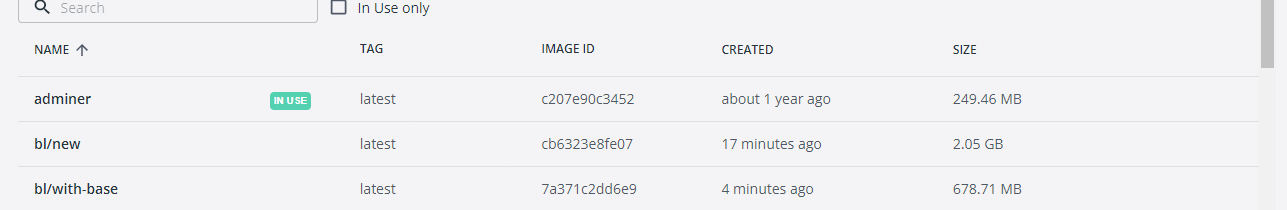
\includegraphics[width=12cm]{report/img/multi_stage.png}\\[10.5cm]
\end{figure}

\subsection{NodeJS}

I servizi UserManagementMaraffa e BusinessLogic sono stati containerizzati utilizzando un'immagine di Node.js. Nell'esempio sotto, si può notare la distinzione tra i diversi stage.
\vspace{1cm}

\begin{lstlisting}[language=Python, caption={Dockerfile delle immagini NodeJS}, label=list:dockerfile_nodejs]
FROM node:20-alpine as base
WORKDIR /app
COPY yarn.lock package.json /app/
RUN yarn install
COPY . /app
RUN yarn build

FROM node:20-alpine
WORKDIR /app    
COPY --from=base /app/package.json /app/package.json
COPY --from=base /app/node_modules /app/node_modules
COPY --from=base /app/dist /app/dist
EXPOSE 3000
CMD ["node","dist/main.js"]
\end{lstlisting}

\subsection{Java}

La containerizzazione del middleware ha richiesto alcuni passaggi aggiuntivi rispetto ai servizi in Node.js.
È stato necessario adottare immagini diverse per gli stage di build e produzione, quindi usare un'immagine di Gradle per la build, nella quale eseguire i comandi di Gradle, e un'immagine di 
OpenJDK per l'esecuzione del JAR prodotto dalla build.

Per la compilazione con Gradle, nonostante non sia una pratica corretta, è stato necessario mantenere nella repository il file gradle-wrapper.jar, in quanto non era possibile scaricarlo durante la build all'interno delle GitHub Actions.
La build non utilizza il classico comando di Gradle per generare il file .jar, ma un task personalizzato che si occupa di generare il fatJar del servizio, poiché le dipendenze non venivano gestite correttamente all'interno del normale file .jar.

\begin{lstlisting}[language=Java, caption={Task del fatJar da includere nel container}, label=list:gradle_fatJar]
tasks.register<Jar>("fatJar") {
    archiveBaseName.set("Middleware")
    manifest {
        attributes["Main-Class"] = "server.Main"
    }
    from(sourceSets.main.get().output)
    dependsOn(configurations.runtimeClasspath)
    from({ configurations.runtimeClasspath.get().filter { it.name.endsWith("jar") }.map { zipTree(it) } })
    dependsOn("compileJava")
    duplicatesStrategy = DuplicatesStrategy.EXCLUDE // Puoi utilizzare altre strategie come DuplicatesStrategy.WARN per avvisare ma non fermare la build
}
\end{lstlisting}

\subsection{Angular}

La containerizzazione del frontend ha richiesto l'utilizzo di un'immagine di Node.js per lo stage di build, mentre per l'esecuzione è stata utilizzata un'immagine di Nginx.
Come citato nella sezione \ref{Nginx} Nginx serve per eseguire l'applicazione all'interno del container e per poterla raggiungere dall'esterno.

    \chapter{Conclusions and Future Work}
\label{ch:con}
\section{Conclusioni}
L'architettura basata su micro-servizi si è rivelata una scelta altamente vantaggiosa per il progetto,
 garantendo modularità, scalabilità e resilienza. Ogni micro-servizio è stato progettato per gestire specifiche
  funzionalità, e la loro integrazione avviene tramite API REST e websocket orchestrate da un middleware centrale, che facilita
   una comunicazione efficiente e ben strutturata tra le componenti del sistema. L'adozione di Docker ha semplificato
    ulteriormente il processo di deploy, offrendo un ambiente di esecuzione coerente e adattabile, capace di gestire le
     diverse esigenze di configurazione e scaling e affidabilità.
% \ref{ch:results} 

L'architettura basata su micro-servizi si è rivelata una scelta altamente vantaggiosa per il progetto,
 garantendo modularità, scalabilità e resilienza. 
  Questo approccio consente una maggiore flessibilità nello sviluppo,
permettendo ai team di lavorare in modo indipendente su componenti diverse, riducendo al contempo le interdipendenze
 e i conflitti di integrazione.

Quest'integrazione avviene tramite API REST e websocket orchestrate da un middleware centrale, che facilita una 
comunicazione efficiente e ben strutturata tra le componenti del sistema. Questo sistema intermediario,
 gestisce le richieste e il bilanciamento del carico, garantendo che i dati siano trasferiti in modo rapido
 tra i vari micro-servizi. Inoltre, l'uso di websocket consente una comunicazione bidirezionale in near real-time,
  migliorando la reattività dell'applicazione.

L'adozione di Docker ha semplificato ulteriormente il processo di deploy, offrendo un ambiente di esecuzione coerente
 e adattabile. Docker, infatti, permette di incapsulare ogni micro-servizio in un container, che include tutte le
  dipendenze necessarie, eliminando problemi legati alle differenze tra ambienti di sviluppo e di test.
Questo approccio non solo facilita la distribuzione, ma migliora anche la portabilità delle applicazioni e la gestione
 delle risorse. Grazie a Docker, è possibile scalare orizzontalmente i micro-servizi in base alle necessità,
 rispondendo rapidamente alle variazioni del carico di lavoro e garantendo così un'elevata disponibilità e affidabilità del sistema.

Infine, l'architettura a micro-servizi, risulta essere altamente resiliente. In caso di fallimento di un singolo micro-servizio,
 il sistema può continuare a funzionare, con la possibilità di isolare e risolvere il problema senza impattare l'intera
  applicazione. Questo approccio modulare non solo migliora la robustezza del sistema, ma facilita anche l'implementazione
   di nuove funzionalità e l'aggiornamento di quelle esistenti, rendendo l'intero processo di sviluppo più agile e
    reattivo.
    

    
   

    
\end{document}
